% !TeX spellcheck = de_DE_igerman98
\documentclass[germanthesis]{thesis-style}
% options:
% [germanthesis] - Thesis is written in German
% [plainunnumbered] - Don't print numbers on plain pages
% [earlydraft] - Settings for quick draft printouts
% [watermark] - Print current time/date at bottom of each page
% [phdthesis] - switch to PhD thesis style
% [twoside] - double sided
% [cutmargins] - text body fills complete page

% Extension to BibLaTex (useful for cites in footnotes)
%\usepackage[backend=bibtex, style=numeric-comp]{biblatex}
\bibliography{references.bib}
%\defbibheading{bibliography}[\refname]{\section*{#1}}


\author{Benedikt~Wimmer}
\title{R-Paket für Kanalkodierung mit Blockkodes}
%\title{R~package for channel~coding with block~codes}
\birthday{1. Feber 1994}
\birthplace{Sonthofen}
%\thesisstart{1. Januar 2009}
\thesistype{Bachelor's thesis}
\thesistypegerman{Bachelorarbeit}
\thesiscite{Bachelor's thesis}
\advisors{Univ.-Prof.~Dr.~Rainer~Böhme, Dr.~Pascal~Schöttle}

% additional packages
\usepackage{color, colortbl} % colors (interface table)
\usepackage{longtable}


%\usepackage[chapter]{algorithm}
%\usepackage[noend]{algpseudocode}
\makeatletter
\def\thm@space@setup{%
  \thm@preskip=\parskip \thm@postskip=0pt
}
\makeatother

% change name of caption by tables
\usepackage{caption}
\captionsetup[longtable]{name=Funktion}

%set listing language to R
\lstset{language=R, prebreak={},} 

\makeatletter
\def\ScaleIfNeeded{%
\ifdim\Gin@nat@width>\linewidth
\linewidth
\else
\Gin@nat@width
\fi
}
\makeatother

\newcommand{\plotwidth}{0.6\textwidth}
\begin{document}

% Titelseiten und Eidesstattliche Erklärung
\maketitle

% Zusammenfassung
\begin{abstract}
Diese Arbeit dokumentiert das R-Paket für Kanalkodierung mit Blockkodes und erläutert die theoretischen Grundlagen und deren Implementierung, sowie die erzeugten Visualisierungen.
\end{abstract}
% Abstract
%\begin{otherlanguage}{american}%
%\begin{abstract}
%
%\end{abstract}
%\end{otherlanguage}

\tableofcontents
\cleardoublepage
\pagenumbering{arabic}

\chapter{Einleitung}
\label{chapter:introduction}
% einleitung.tex
Kanalkodierung stellt, aufgrund der stetigen Ausbreitung digitaler Kommunikationssysteme, ein wichtiges Teilgebiet der Kodierungstheorie dar. Informationen, die über einen Kanal zwischen Quelle und Empfänger übertragen werden, können aufgrund von Rauschen verändert werden. Die Kanalkodierung stellt Methoden zur Verfügung, um Fehler, die während der Übertragung über einen verrauschten Kanal auftreten, zu korrigieren. Verwendung findet die Kanalkodierung in der Mobil- und Satellitenkommunikation, da beispielsweise das erneute Senden von Satellitendaten, bei Auftreten von Rauschen, aufgrund der Laufzeiten unpraktisch wäre. Weiters wird die Kanalkodierung zur Speicherung von Daten, etwa auf Compact-Disks, verwendet. Rauschen kann durch thermische Störungen bzw. Kratzer oder Fingerabdrücke auf Compact-Disks hervorgerufen werden.

Eine Art der Kanalkodierung stellen Faltungskodes dar, auf welche sich diese Arbeit konzentriert. Die wichtigste Anwendung von Faltungskodes ist die Konstruktion von Turbo-Kodes, welche eine Erweiterung der Faltungskodes darstellen. Weiters existiert mit Blockkodes ein weiteres wichtiges Verfahren der Kanalkodierung.
\\
\\
Ziel dieser Arbeit ist die Implementierung von Faltungskodes mithilfe der Programmiersprache R. Das entwickelte R-Paket dient zukünftigen Studierenden zu Lehrzwecken und soll sie beim Studieren von Faltungskodes unterstützen. Studierenden soll dadurch, neben den theoretischen Grundlagen im Zuge einer Vorlesung, eine praktische Möglichkeit zur Anwendung von Faltungskodes geboten werden. Mithilfe dynamisch generierter Visualisierungen, sollen die Prinzipien von Faltungskodes vermittelt werden.

Die Arbeiten \enquote{R-Paket für Kanalkodierung mit Blockkodes}~\cite{wimmer} von Benedikt Wimmer und \enquote{R-Paket für Kanalkodierung mit Turbo-Kodes}~\cite{witsch} von Daniel Witsch stellen Implementierungen der Blockkodes bzw. Turbo-Kodes zur Verfügung, die ebenfalls im Paket enthalten sind. Dadurch ergibt sich ein sowohl umfangreiches als auch kompaktes Paket der Kanalkodierung.




\startlist[tables]{lot}
\chapter{Grundlagen und verwandte Arbeiten}
\label{chapter:theory}
%theory.tex


Um die Funktionsweise der Blockkodes auf mathematischer Ebene zu erklären müssen zunächst einige Definitionen gemacht werden. Diese Eigenschaften haben alle im Folgenden genauer erklärten Kodes gemeinsam.
\newtheorem{t_def}{Definition}[chapter]

\begin{t_def}
Ein {\em Datenwort d} wird durch die Anwendung eines {\em Kodes C} zum {\em Kodewort c}.
\end{t_def}

Da wir uns auf binäre Kodes beschränken sind alle Kode- und Datenwörter eine Konkatenation aus 0en und 1en, oder mathematisch formuliert:

\begin{t_def}
Der binäre Körper $\mathbb{F}_{2}$ ist ein endlicher Körper $\mathbb{F}_{q}$ bestehend aus den Elementen \{0,1\}
\end{t_def}

Obige Definition entspricht auch $\mathbb{Z}_2$, dem Restklassenring $\mathbb{Z}\mod 2$. Eine andere Bezeichnung für einen endlichen Körper ist das Galois-Feld, geschrieben als GF(q) bzw. GF(2) für den binären Körper. Daraus ergibt sich für die Addition und Multiplikation:\newline

\begin{table}[!h]
\begin{center}
\begin{tabular}{c|cc}
+ & 0 & 1 \\
\hline
0 & 0 & 1 \\
%\hline
1 & 1 & 0 \\
\end{tabular}
\hspace{2cm}
\begin{tabular}{c|cc}
$\cdot$ & 0 & 1 \\
\hline
0 & 0 & 0 \\
%\hline
1 & 0 & 1 \\
\end{tabular}
\caption{Addition und Multiplikation in $\mathbb{F}_2$}
\label{table:addmul}
\end{center}
\end{table}

Sofern nicht anderst angegeben beziehen sich Rechenoperationen auf Kode- und Datenwörtern immer auf den Körper $\mathbb{F}_2$. Deswegen gibt es semantisch gesehen auch keinen Unterschied zwischen Addition und Subtraktion da $\{-x = x \mid x \in \mathbb{F}_2\}$.\cite[Kap. 1.1]{huffman2010fundamentals}

\begin{t_def}
$\mathbb{F}_{2}^{n}$ ist der Vektorraum aller {\em n-Tupel} über dem Körper $\mathbb{F}_2$.
\end{t_def}


\begin{t_def}[Lineare Kodes]
Ein {\em Kode C} mit Kodewörtern der Länge n ist genau dann {\em linear}, wenn er ein Untervektorraum von $\mathbb{F}_{2}^{n}$ ist.
\end{t_def}

Alle in dieser Arbeit behandelten Kodes gehören zur Klasse der \textit{linearen Kodes}.\cite[Kap. 1.2]{huffman2010fundamentals} Um nun deren Fehlerkorrektureigenschaften zu betrachten muss noch der Begriff der Hamming-Distanz definiert werden.

\begin{t_def}
Die {\em Hamming Distanz h} zwischen 2 Kodewörtern $x,y \in \mathbb{F}_{2}^{n}$ ist definiert als die Anzahl der Stellen i für die gilt: $x_i \neq y_j$
\end{t_def}

Dies bedeutet, wenn die Kodewörter in einem Kode C eine Hamming-Distanz von $h=1$ zueinander haben, dann unterscheiden sich die Kodewörter nur in einer Stelle voneinander. Das heißt sobald 1 Fehler passiert wird direkt ein anderes, gültiges Kodewort getroffen und der Fehler wird nicht erkannt. Auch $h=2$ reicht noch nicht aus um einen Fehler zu korrigieren. Man erhält zwar ein ungültiges Kodewort, kann aber nicht sagen welches es vor dem Fehler war. Um einen 1-Bit-Fehler zu korrigieren benötigt man also einen Kode mit mindestens $h=3$.\cite[Kap. 1.4]{huffman2010fundamentals} Daraus resultiert folgende Definition:

\begin{t_def}
In einem t-Fehler korrigierenden Kode brauchen alle Kodewörter mindestens eine Hamming-Distanz von $h=2t+1$ zueinander.
\end{t_def}


\section{Hamming-Kodes}
\label{section:hamming}

Die wohl simpelsten Blockkodes sind die Klasse der Hamming-Kodes. Ein Hamming-(n,k)-Kode erzeugt Kodewörter c der Länge n für die gilt: $c \in \mathbb{F}_{2}^{n}$ aus Datenwörtern d der Länge k für die gilt: $d \in \mathbb{F}_{2}^{k}$. Ein Hamming-Kode hat eine Hamming-Distanz von $h=3$ und kann somit 1-Bit-Fehler korrigieren. Gültige (n,k)-Tupel erfüllen die Gleichungen $r = n - k$ und $n = 2^r - 1$.\cite[Kap. 1.8]{huffman2010fundamentals} Die Kodierung und Dekodierung erfolgt mittels jeweils einer Generator- und Kontrollmatrix.

\begin{t_def}
Für eine Generatormatrix G eines Kodes C mit Kodewörtern c und Datenwörtern d gilt: $ dG = c$
\end{t_def}

\begin{t_def}
Für eine Kontrollmatrix H eines Kodes C gilt: $ Hx^T = 0$ genau dann, wenn $x \in C$.
\end{t_def}

Obige Definitionen gelten für alle lineare Kodes\cite[Kap. 1.2]{huffman2010fundamentals}, aber anderst als bei den BCH-Kodes werden bei den Hamming-Kodes die Matrizen direkt zur En- und Dekodierung verwendet.

\begin{t_def}
Ein {\em systematischer} Kode enthält das Datenwort in Reinform.
\end{t_def}

Alle in dieser Arbeit verwendeten Kodes sind systematisch, da dies die Nachvollziehbarkeit im Rahmen des Lehrzweckes verbessert. Um einen systematischen Hamming-Kode zu erzeugen, müssen die Generatormatrix G und die Kontrollmatrix H folgende Standardform\cite[Kap. 1.1.3]{morelos2006art} haben: 

$$G = \left(I_k \mid A\right)$$
$$H = \left(A^T \mid I_r\right)$$

Um die Matrizen zu konstruieren muss man H genauer betrachten. Der Spaltenraum von H entspricht den r-Tupeln der Zahlen 1,2,...,n in Binärdarstellung. H kann nun durch Spaltenumformungen in Standardform gebracht werden. 
Anschließend kann G durch transponieren von A nach obiger Gleichung erzeugt werden.\cite[Kap. 1.8]{huffman2010fundamentals} Hier ein Beispiel für einen Hamming-(7,4)-Kode:

$$r = n-k = 3$$
$$H' = \begin{pmatrix}
0 & 0 & 0 & 1 & 1 & 1 & 1 \\
0 & 1 & 1 & 0 & 0 & 1 & 1 \\
1 & 0 & 1 & 0 & 1 & 0 & 1 \\
\end{pmatrix}\text{\qquad{1,2,...,7}}$$

$$H = \begin{pmatrix}
0 & 1 & 1 & 1 & 1 & 0 & 0 \\
1 & 0 & 1 & 1 & 0 & 1 & 0 \\
1 & 1 & 0 & 1 & 0 & 0 & 1 \\
\end{pmatrix}\qquad{(A^T \mid I_r)}$$

$$G = \begin{pmatrix}
1 & 0 & 0 & 0 & 0 & 1 & 1 \\
0 & 1 & 0 & 0 & 1 & 0 & 1 \\
0 & 0 & 1 & 0 & 1 & 1 & 0 \\
0 & 0 & 0 & 1 & 1 & 1 & 1 \\
\end{pmatrix}\qquad{(I_k \mid A)}$$

Semantisch betrachtet beschreibt die Generatormatrix ein Gleichungssystem für die Paritätsbits. Die Spalten der Einheitsmatrix beschreiben die trivialen Gleichungen $d_i = d_i$, die Spalten von A beschreiben jeweils die Gleichung eines Paritätsbits. Für ein Datenwort $d=(a,b,c,d)$ ergeben sich für die Paritätsbits $p=(e,f,g)$ des resultierenden Kodeworts $c=(a,b,c,d,e,f,g)$ nach der Kodierung durch $dG = c$ folgende Gleichungen:

$$ e = b+c+d$$
$$ f = a+c+d$$
$$ g = a+b+d$$

Stimmen alle Gleichungen, dann liegt ein gültiges Kodewort vor. Ist nur eine Gleichung falsch, muss es das dazugehörige Paritätsbit sein. Sind alle falsch, muss es d sein. Sind 2 falsch, dann muss das Bit sein welches in beiden Gleichungen vorkommt. Genau diese Informationen Stecken in der Kontrollmatrix H. Ein Vektor des Spaltenraums von H[,i] beschreibt ein "Fehlermuster" in den Gleichungen, seine Position i das verursachende Fehlerbit im Kodewort. Eine allgemeiner Ansatz zum Dekodieren:

\begin{itemize}
\item Wenn $Hc^T = 0$, dann ist kein Fehler passiert.
\item Anonsten ist an Position i für $Hc^T = H[ ,i]$ der Fehler passiert.
\end{itemize}

Daraus resultiert auch, dass ein 2. Fehler nicht erkannt wird, da alle möglichen r-Tupel, die bei einer Multplikation mit H entstehen können, bereits definiert sind. 


\section{BCH-Kodes}

Die \textbf{B}ose, Ray-\textbf{C}haudhuri, \textbf{H}ocquenghem bilden eine wichtige Klasse der linearen Kodes. Des weiteren gehören sie zu den polynomiellen und zyklischen Kodes.\cite[Kap. 5.1]{huffman2010fundamentals}
Ein (n,k,d)-BCH-Kode hat n-Bit lange Kodewörter, k-Bit lange Datenwörter und eine minimale Hamming-Distanz von $d = 2*t+1$.
Grundsätzlich werden hier die Daten- und Kodewörter als Polynome interpretiert. Da wir uns weiterhin auf binäre Kodes beschränken sind die Koeffizienten der Polynome aus 
$\mathbb{F}_{2}$, es gelten die in \ref{section:hamming} definierten Eigenschaften. Daraus ergibt sich zum Beispiel $x^3 -x -1 \equiv x^3 + x + 1$. Das Datenwort 1011 wird interpretiert als $x^3 + x^2 + 1$. Es folgen einige nötige Definitionen:

\begin{t_def}
Sei $n \in \mathbb{N}$ die Länge der Kodewörter und $m \in \mathbb{N}$ die kleinste Zahl für die gilt: $n \leq 2^m -1$, dann ist $\mathbb{F}_{2^m}$ eine Körpererweiterung des endlichen Körpers $\mathbb{F}_{2}$
\end{t_def}

Diese Körpererweiterung wird auch bezeichnet als $GF(2^m)$. 
Es existiert ein \textit{primitives Element} $\alpha \in GF(2^m)$ für das gilt: Für jedes $\beta \in GF(2^m)\setminus\{0\}$ gilt: $\beta = \alpha^j$ für $0 \leq j \leq 2^m -2$ und $n = 2^m-1$ ist die kleinste positive Zahl für die gilt: $\alpha^n = 1$. Oder anderst ausgedrückt: $\alpha$ ist die {\em primitive n-te Einheitswurzel}.\cite[Kap. 3.2.1]{morelos2006art}
Nun existiert ein irreduzibles Polynom p(x) von Grad m für das gilt: $p(\alpha) = 0$, somit ist es ein {\em primitives Polynom}.

\begin{t_def}
Seien $F(x)$ alle Polynome mit Koeffizienten aus $\mathbb{F}_2$ und $p(x)$ ein primitives Polynom zu $GF(2^m)$, dann sind die Elemente von $GF(2^m)$ die Restklassen von $F(x) \mod p(x)$.  \cite[Kap. 5.2]{bose2008infotheory}
\end{t_def}

Eine weitere Darstellung der Elemente in $GF(2^m)$ ist die als binärer Vektor der Länge m. Es folgt ein Beispiel zur Veranschaulichung der 3 Darstellungen von $GF(2^m)$, den Potenzen von $\alpha$, den polynomiellen Restklassen und den korrespondierenden Binärdarstellungen. Für $m=3$ und $p(x) = x^3 + x + 1$ erhält man:


\begin{table}[!h]
\begin{center}
\begin{tabular}{c|c|c}
$\alpha^i$ & Polynom & Vektor \\
\hline
- & 0 & 000 \\
$\alpha^0$ & $1$ & 001 \\
$\alpha^1$ & $x$ & 010 \\
$\alpha^2$ & $x^2$ & 100 \\
$\alpha^3$ & $x+1$ & 011 \\
$\alpha^4$ & $x^2+x$ & 110 \\
$\alpha^5$ & $x^2+x+1$ & 111 \\
$\alpha^6$ & $x^2+1$ & 101 \\
\end{tabular}
\caption{$GF(8)$}
\label{table:gf}
\end{center}
\end{table}




Die Vektordarstellung ist hauptsächlich für die Implementierung relevant, da dies das Rechnen mit den Polynomen vereinfacht. Eine Addition von $a+b \mid a,b \in GF(2^m)$ entspricht $v_a \oplus v_b$ für $v_a,v_b$ in Vektordarstellung. Multiplikation entspricht einer Addition der Potenzen von $\alpha \mod 2^m-1$, also zum Beispiel $\alpha^3\alpha^5 = \alpha^8 = \alpha^1$.\cite[Kap. 3.2.1]{morelos2006art}

\begin{t_def}
Das Minimalpolynom $\phi_i(x)$ eines Elements $\alpha^i$ ist das Polynom kleinsten Grades mit $\phi_i(\alpha^i) = 0$.\cite[Kap 3.2.1]{morelos2006art}
\end{t_def}

Um die Minimalpolynome für jedes $\alpha^i$ zu bestimmen muss man zunächst die Menge aller Zykel $C_s$ $\mod 2^m-1$ ermitteln. Diese sind für das obere Beispiel folgende:

\begin{center}
$$C_0 = \{0\}, C_1 = \{1,2,4\}, C_3 = \{3,6,5\}$$
\end{center}

\begin{t_def}
Für jeden Zykel s in der Menge aller Zykel ist das Minimalpolynom definiert als: $$\phi_s(x) = \prod_{i_s \in C_s}(x+\alpha^{i_s})$$\cite[Kap. 3.2.1]{morelos2006art}
\end{t_def}

Aus obiger Definition ergibt sich, dass jeweils die Potenzen von $\alpha$, die Elemente des selben Zykels sind, dasselbe Minimalpolynom besitzen. Dadurch können wir die Tabelle~\ref{table:gf} erweitern:

\begin{table}[!h]
\begin{center}
\begin{tabular}{c|c|c|c}
$\alpha^i$ & Polynom & Vektor & Minimalpolynom\\
\hline
- & 0 & 000 & - \\
$\alpha^0$ & $1$ & 001 & - \\
$\alpha^1$ & $x$ & 010 & $x^3+x+1$ \\
$\alpha^2$ & $x^2$ & 100  & $x^3+x+1$ \\
$\alpha^3$ & $x+1$ & 011  & $x^3+x^2+1$ \\
$\alpha^4$ & $x^2+x$ & 110  & $x^3+x+1$ \\
$\alpha^5$ & $x^2+x+1$ & 111  & $x^3+x^2+1$ \\
$\alpha^6$ & $x^2+1$ & 101  & $x^3+x^2+1$  \\
\end{tabular}
\caption{$GF(8)$ mit Minimalpolynomen}
\label{table:minimals}
\end{center}
\end{table}

Eine ausführliche Herleitung für Berechnung der Minimalpolynome findet sich in \cite[Kap. 3.2.1]{morelos2006art}.

\begin{t_def}
Sei t die Anzahl der zu korrigierenden Fehler und LCM das kleinste gemeinsame Vielfache. Dann ist das Generatorpolynom definiert als:
$$g(x) = LCM(\phi_1(x),\phi_2(x),...,\phi_{2t}(x))$$
\end{t_def}

So ergibt sich aus Tabelle~\ref{table:minimals} und $t=3$ das Generatorpolynom:
$$g(x) = LCM(\phi_1(x),\phi_2(x)) = LCM((x^3+x+1)(x^3+x+1)) = x^3+x+1$$

Dies ist ein BCH-(7,4,3)-Kode, es entpsricht der zyklischen Version eines Hamming-(7,4)-Kodes. Ein Generatorpolynom für jeden binären BCH-Kode kann auf diese Weise ermittelt werden.

\begin{t_def}
Sei d(x) ein Datenpolynom der Länge k und g(x) das Generatorpolynom eines BCH-(n,k,d)-Kodes. Dann ist das resultierende Kodewort definiert als:
$$k(x) = d(x)x^{n-k} - d(x)x^{n-k} \mod g(x)$$
\end{t_def}

Für den (7,4,3)-Kode aus Tabelle~\ref{table:minimals} mit Generatorpolynom $x^3+x+1$ ergibt sich also folgende Kodierung für ein Datenwort $d(x)$:

$$d(x) = 1011$$
$$d(x) = x^3 + x^2 + 1$$
$$d'(x) = d(x)x^3 = x^6 + x^5 + x^3$$
$$k(x) = d'(x) - d'(x) \mod g(x)$$
$$k(x) = d'(x) + 1 = x^6 + x^5 + x^3 + 1$$
$$k(x) = 1001011$$

Um die Schritte nachzurechnen sollte man stets die Eigenschaften der Koeffizienten aus $\mathbb{F}_2$, definiert in Tabelle~\ref{table:addmul}, berücksichtigen.
Wie man sieht handelt es sich auch hier um ein systematisches Kodewort, das Datenwort ist darin enthalten.
\newblock
\newline
Das Dekodieren der BCH-Kodes kann auf verschiedene Arten erfolgen und ist sehr detailliert in Robert Morelos-Zaragoza's "The Art of Error Correcting Coding"(Kapitel 3.5) beschrieben.\cite{morelos2006art}
An dieser Stelle folgt eine kurze Zusammenfassung der relevanten Schritte.
Die Dekodierung der BCH-Kodes erfolgt im allgemeinen in 4 Stufen:

\begin{enumerate}
\item Berechnen der Syndrome $S_i = k(\alpha^i) \mid 1 \leq i \leq 2t$
\item Bestimmem des Fehlerstellenpolynoms $\sigma(x)$.
\item Ermitteln der Inversen der Nullstellen von $\sigma(x)$, diese entsprechen den Fehlerindizes $\alpha^i$
\item Korrigieren der Fehler im Kodewort und den Fehlerindizes.
\end{enumerate}

Die Syndrome sind die Auswertung des erhaltenen Kodeworts $k(x)$ an den Nullstellen $\alpha^{1,...,2t}$. 
Für das Kodewort $k(x) = 1001011 = x^6 + x^5 + x^3 + 1$, $t=2$ und $GF(8)$ aus Tabelle~\ref{table:gf} ergeben sich folgende Syndrome:

$$S_1 = k(\alpha^1) = \alpha^6 + \alpha^5 + \alpha^3 + 1 = (x^2 +1) + (x^2+x+1)(x+1)+1 = 0$$
$$S_2 = k(\alpha^2) = \alpha^{12} + \alpha^{10} + \alpha^6 + 1 = \alpha^5 + \alpha^3 + \alpha^6 + 1 = 0 $$

Da unser Kodewort keine Fehler enthielt sind die Syndrome $S_i = 0$. Wenn es nur darum geht Fehler zu erkennen wäre dieser Schritt bereits ausreichend. Für ein Fehlerhaftes Kodewort $k'(x) = 1101011 = x^6 + x^5 + x^3 + x+1$ ergeben sich die Syndrome: 
$$S_1 = 0 + \alpha^1 = x$$
$$S_2 = 0 + \alpha^2 = x^2$$

Um nun die Fehlerindizes zu bestimmen muss zunächst das Fehlerstellenpolynom $\sigma(x)$ mit Hilfe des Berlekamp-Massey-Algorithmus ermittelt werden. Dieser ist in \cite[Kap 3.5.2]{morelos2006art} beschrieben. Für das Fehlerhafte Kodewort $k'(x)$ liefert dieser $\sigma(x) = \alpha x +1$. Ist der Grad von $\sigma(x) > t$ sind mehr als t Fehler im Kodewort und es kann nicht vollständig dekodiert werden. In diesem Fall ist $deg(\sigma(x)) = t$, also müssen nun die Inversen der Nullstellen von $\sigma(x)$ bestimmt werden. Das verwendete Verfahren nennt sich Chien's Suche, dabei wird für alle $\beta \in GF(2^m)\setminus\{0\}$ die Bedingung $\sigma(\beta^{-1}) = 0$ überprüft.\cite[Kap. 3.5.5]{morelos2006art} Für $\sigma(x) = \alpha x +1$ ergibt sich:

$$\sigma(\alpha^6) = \alpha^1\alpha^6 +1 = \alpha^7 +1 = \alpha^0 + 1 = 1 + 1 = 0$$

Da $\alpha^{-6} = \alpha^1$ ist haben wir den Fehler in $k'(x) = 1101011 = x^6 + x^5 + x^3 + x+1$ an Index 1 indentifiziert.

$$k'(x) - x = x^6 + x^5 + x^3 + x+1 -x = x^6+x^5+x^3+1=k(x)$$



\subsection{Reed-Solomon-Kodes}

Die Klasse der Reed-Solomon-Kodes, kurz RS-Kodes, findet viele Anwendungen im Bereich der digitalen Datenspeicherung auf CDs und DVDs, sowie in Kommunikationssystemen.\cite[Kap. 4]{morelos2006art} Die hierfür verwendeten Kodes sind allerdings nicht mehr binär und daher für die Simulation in dieser Arbeit nicht verwendbar. Die binären RS-Kodes bilden eine Unterklasse der binären BCH-Kodes mit einer Einschränkung: Die Länge der Kodewörter ist $n = 2^m-1$.\cite[Kap 5.2]{huffman2010fundamentals} Dadurch ist der einzige Unterschied im binären, dass BCH-Kodes flexibler in der Kodelänge sind. Gerade für nicht-binäre RS-Kodes ergeben sich aber Vereinfachungen im Bestimmen des Generatorpolynoms und dem Dekodieren, dies ist in \cite[Kap. 4]{morelos2006art} und \cite[Kap. 5.2]{huffman2010fundamentals} gut beschrieben.

\stoplist[tables]{lot}

\startlist[Funktionen]{lot}
\chapter{Implementierung}
\label{chapter:implementation}
% implementierung.tex
Dieses Kapitel gibt einen Einblick in die Konzepte der Implementierung. Als Einstiegspunkt stand eine Referenzimplementierung\footnote{\url{http://vashe.org/turbo/turbo_example.c} (01.06.2016)} zur Verfügung, die den Dekodier-Algorithmus für Turbo-Kodes beinhaltet, jedoch für ein konkretes Beispiel. Dieser musste angepasst werden um für allgemeine Faltungskodes verwendbar zu sein.
\\
\\
Kapitel \ref{kapitel:implementierung_faltungskodierer} beinhaltet den Entwurf der Faltungskodierer-Datenstruktur. [TODO: Fertigstellung]
%Die Implementierung der Kodierung wird in Kapitel \ref{kapitel:implementierung_kodierung} beschrieben, die der Dekodierung in Kapitel \ref{kapitel:implementierung_dekodierung}.
%\\
%\\
%Aus Performancegründen Kodierung, Dekodierung in C++\\
%Weiters: Kodierer erzeugen, Depunktierung, Katastrophale Kodierer Prüfung (Polynom GGT mod 2)
%\\
%Parameterprüfung, Punktierung, ApplyNoise, Aufruf Visualisierung in R\\
%Referenzimplementierung
\section{Faltungskodierer}
\label{kapitel:implementierung_faltungskodierer}
Ein Faltungskodierer ist gegeben durch 
\begin{itemize}
\item $N$: Anzahl an Ausgangsbits je Eingangsbit,
\item $M$: Länge des Schieberegisters,
\item $G$: Vektor von Generatorpolynomen.
\end{itemize}
Die Angabe von $M$ ist hier redundant, jedoch Teil der Benutzereingabe zur Generierung eines Faltungskodierers, welche durch \cite{morelos2006art} inspiriert wurde.
\\
\\
Zur leichteren Implementierung der Kodierung und Dekodierung wird die Kodierer-Datenstruktur um folgende Elemente erweitert:
\begin{itemize}
\item eine \emph{Zustandsübergangsmatrix}, die angibt, in welchen Zustand der Kodierer bei einem Eingangsbit wechselt,
\item eine \emph{inverse Zustandsübergangsmatrix}, die angibt, aus welchem Zustand der Kodierer bei einem Eingangsbit kommt,
\item eine \emph{Ausgabematrix}, die angibt, welche Kodebits der Kodierer bei einem Eingangsbit in einem bestimmten Zustand ausgibt,
\item ein Flag zur Markierung rekursive systematischer Kodierer (RSC, siehe Kapitel~\ref{kapitel:grundlagen_rsc}),
\item ein \emph{Terminierungsvektor} die für rekursiver systematische Kodierer angibt, ob ein Eingangsbit 0 oder 1 in einem bestimmten Zustand für die Terminierung zu verwenden ist.
\end{itemize}
Die Implementierung der Matrizen wurde aus der Referenzimplementierung übernommen, musste jedoch erweitert werden, um für allgemeine Faltungskodes verwendbar zu sein. Für alle gilt, die Anzahl an Zeilen entspricht der Anzahl an Zuständen $2^{M}$. Der Zeilenindex entspricht dem Zustand. Die Zustandsübergangsmatrix sowie die Ausgabematrix besitzen jeweils zwei Spalten. Je eine Spalte steht für ein Eingangsbit (0 oder 1), wobei der Spaltenindex dem Eingangsbit entspricht. Die inverse Zustandsübergangsmatrix benötigt eine dritte Spalte. Für viele Kodierer (v.a. nicht-rekursive) tritt der Fall ein, dass nur durch \emph{ein bestimmtes} Eingangsbit in einen bestimmten Zustand gewechselt werden kann. Sei ein Zustand bspw. nur durch das Eingangsbit 0 erreichbar, so bedeutet das, dass es für diesen Zustand mit dem Bit 0 \emph{zwei} Vorgängerzustände gibt, für ein Eingangsbit 1 jedoch keinen Vorgänger. Diese zweite Möglichkeit wird in der dritten Spalte gespeichert.
\\
\\
Der Terminierungsvektor ist für nicht-rekursive Kodierer nicht notwendig, da ein Kode eines solchen Kodierers immer mit $M$ 0-Bits terminiert wird. Bei einem rekursiven Kodierer ist es nicht trivial zu sagen mit welchem Eingangsbit in einem bestimmten Zustand terminiert wird, um den Kodierer in den Nullzustand zu bringen. Dies hängt von der Definition des Rekursionpolynoms ab. Der Terminierungsvektor wird bei der Erzeugung rekursiver Kodierer berechnet.
\\
\\
Bei der Erzeugung von Faltungskodierern ist zu prüfen ob es sich um einen katastrophalen Kodierer handelt. RSC-Kodierer sind, wie in Kapitel \ref{kapitel:grundlagen_systematische_kodierer} beschrieben, nicht zu prüfen. Zur Prüfung wird nach dem Theorem von Massey-Sain (siehe Kapitel~\ref{kapitel:grundlagen_katastrophale_kodierer}) der größte gemeinsame Teiler der Generatorpolynome berechnet. Die Berechnung des größten gemeinsamen Teilers wurde mithilfe des euklidschen Algorithmus implementiert. Sowohl der euklidsche Algorithmus als auch die dafür notwendige binäre Polynomdivision wird an eine C++-Funktion delegiert.

\section{Kodierung}
\label{kapitel:implementierung_kodierung}
Bei Faltungskodes stellt die Kodierung den bei Weitem einfacheren Teil dar. Es muss lediglich jedes Bit der zu kodierenden Nachricht zusammen mit dem aktuellen Zustand, der nach jedem Bit mithilfe der Zustandsübergangsmatrix aktualisiert wird, auf die Ausgabematrix angewendet werden. Die Terminierung funktioniert analog, einzig das zu kodierende Bit muss ermittelt werden. Für RSC-Kodierer muss im Terminierungsvektor nachgeschaut werden, andernfalls ist das Terminierungsbit immer 0. Abgeschlossen wird die Kodierung mit dem Abbilden der Kodebits 0 bzw. 1 auf die Signalwerte +1 bzw. -1 nach Gleichung~\eqref{eq:bit_zu_signal_abbildung}. Algorithmus~\ref{algorithmus:kodierung} zeigt den Kodierungsalgorithmus.

\begin{algorithm}[H]
\renewcommand{\algorithmicforall}{\textbf{for each}}
\caption{Faltungskodierung}
\label{algorithmus:kodierung}
\begin{algorithmic}[1]
\STATE state $=0$, code $=$ result $=$ " "
\FORALL {bit \textbf{in} message}
   \STATE output $=$ output.matrix[state][bit]
	\STATE code $=$ $concat($code, output$)$
	\STATE state $=$ state.transition.matrix$[$state$][$bit$]$
\ENDFOR
\IF{terminate code}
   \FOR {$i=0$ \TO $M-1$}
      \STATE termination.bit $=$ rsc-coder $?$ termination.vector$[$state$]$ : $0$
      \STATE output $=$ output.matrix$[$state$][$termination.bit$]$
	   \STATE code $=$ $concat($code, output$)$
	   \STATE state $=$ state.transition.matrix$[$state$][$termination.bit$]$
   \ENDFOR
\ENDIF
\FORALL {bit \textbf{in} code}
   \STATE signal $=1-2$bit
   \STATE result $=$ $concat($result,signal$)$
\ENDFOR
\RETURN result
\end{algorithmic}
\end{algorithm}

\section{Dekodierung}
\label{kapitel:implementierung_dekodierung}
Die Dekodierung stellt den wesentlich komplexeren Teil der Faltungskodes dar. 

\begin{algorithm}[H]
\renewcommand{\algorithmicforall}{\textbf{for each}}
\caption{Faltungsdekodierung}
\label{algorithmus:dekodierung}
\begin{algorithmic}[1]
\STATE $NUM_STATES=2^{M}$
\FOR {$t=1$ \TO $length($message$)$}
   \FOR {$s=0$ \TO $NUM_STATES-1$}
   	\STATE $m_{1}=$ metric[t-1][prev.state1] + $\delta_{1}$
   	\STATE $m_{2}=$ metric[t-1][prev.state2] + $\delta_{2}$
      \STATE metric[t][s] = $min(m_{1},m_{2})$
      \STATE survivor.bit $=$ $xyz(0,1,min(min(m_{1},m_{2}))$
	\ENDFOR
\ENDFOR
\RETURN result
\end{algorithmic}
\end{algorithm}

\section{Rauschen}
\label{kapitel:implementierung_noise}
Um auch zeigen zu können, dass die Dekodierung auch tatsächlich für verrauschte Signale funktioniert, benötigt es eine Funktion, die die Übertragung einer Nachricht über einen verrauschten Kanal simuliert, d.h. das Signal mit Rauschen überlagert. Zum Signal soll ein additives weißes gaußsches Rauschen (AWGR oder AWGN\footnote{additive white Gaussian noise}) addiert werden um dieses zu verfälschen. [apply noise quelle] stellt eine alternative Implementierung zur eingebauten AWGN-Funktion in Matlab vor. Die Implementierung wurde übernommen bzw. nach R übersetzt. Durch die Möglichkeit das Signal-Rausch-Verhältnis über einen Parameter zu steuern, können verschiedene Übertragungskanäle simuliert und Nachrichten somit verschieden stark verrauscht werden. Der Benutzer kann dadurch herausfinden, ab wann eine Nachricht zu viel Rauschen enthält, um sie korrekt dekodieren zu können. Weiters kann nach mehrfacher Ausführung auf Fehlermuster geschlossen werden, mit denen die Dekodierung gut bzw. schlecht umgehen kann. Durch Versuche mit anderen Kanalkodierungs-Methoden können Vergleiche mit diesen angestellt werden. Die genannten Punkte helfen dem Benutzer sein Verständnis für Faltungskodes noch besser zu stärken.

\section{Punktierung}
\label{kapitel:implementierung_punktierung}
Punktierung leicht, jedoch Depunktierung vor der Dekodierung nicht trivial.

%\section{Visualisierung}
%\label{kapitel:implementierung_visualisierung}
\stoplist[Funktionen]{lot}

\chapter{Visualisierung}
\label{chapter:visualization}
% visualisierung.tex
Wird der \texttt{visualize}-Parameter bei der Ausführung einer R-Paket-Funktion auf \texttt{TRUE} gesetzt, wird ein \texttt{RMarkdown}-Skript ausgeführt. Dieses generiert eine  Präsentation vom \LaTeX -Dokumenttyp \emph{Beamer} mit Informationen und Visualisierungen zur ausgeführten Funktion.
\\
Die erzeugten Präsentationen liegen innerhalb des Programmverzeichnisses von R im Installationsordner des Pakets. Dort gibt es den Ordner \emph{pdf}, in dem sich die Dokumente befinden. Möchte man die Dokumente von RStudio aus öffnen, anstatt die Dokumente in der Verzeichnisstruktur suchen zu müssen, kann die \texttt{ConvOpenPDF}-Funktion (siehe Funktion~\ref{funktion:ConvOpenPDF}) verwendet werden. Möchte man die Dokumente zu einem späteren Zeitpunkt erneut einsehen, wird empfohlen eine Kopie der Datei abzuspeichern, da bei einer erneuten Ausführung der gleichen Funktion inklusive Visualisierung das zuvor erzeugte Dokument im \emph{pdf}-Ordner überschrieben wird. Die vom \texttt{RMarkdown}-Skript erzeugten \LaTeX -Dateien, aus denen die Beamer Präsentationen generiert werden, liegen ebenfalls im selben Verzeichnis.
\\
Da einerseits der Platz auf einer Folie begrenzt ist und andererseits Visualisierungen zu Lehrzwecken nur für kurze Bitsequenzen sinnvoll sind, gibt es Einschränkungen für die in einer Visualisierung verwendeten Nachrichten und Kodierer. Eine Visualisierung der Kodierung bzw. Dekodierung erfolgt für Nachrichten bzw. dekodierte Nachrichten inklusive Terminierungsbits bei einer Länge von bis zu 14 Bits. Bei einem Faltungskodierer mit einer Schieberegisterlänge von vier oder größer erfolgt keine Visualisierung der Dekodierung, da das Trellis zu groß ist. Bei der Kodierung wird nur das Zustandsdiagramm nicht abgebildet.
\\
Bei den folgenden Beispielen der Visualisierungen wurde stets punktiert, da ohne Punktierung die Informationen zur Punktierung in den Präsentationen fehlen und somit auch nicht erläutert werden können.
\\
\\
Der weitere Kapitelinhalt setzt sich folgendermaßen zusammen: Die Kapitel~\ref{kapitel:visualisierung_kodierung} bzw. \ref{kapitel:visualisierung_dekodierung} beinhalten Erläuterungen zur Visualisierung der Kodierung bzw. Dekodierung. Kapitel~\ref{kapitel:visualisierung_simulation} beschreibt die Visualisierung der Simulation.
\section{Kodierung}
\label{kapitel:visualisierung_kodierung}
% allg. Informationen
Bei der Kodierung befinden sich auf den ersten Folien allgemeine Informationen zum verwendeten Faltungskodierer. Abbildung~\ref{abb:folie_kodierer_kennwerte} zeigt die Folie mit den Kennwerten des Faltungskodierers: Anzahl an Ausgängen $N$, Länge des Schieberegisters $M$, Generatorpolynome, Punktierungsmatrix und Koderate. Auf den nächsten beiden Folien werden die Zustandsübergangsmatrix und die Ausgabematrix abgebildet. In Abbildung~\ref{abb:folie_zustandsübergangsmatrix} ist die Folie der Zustandsübergangsmatrix zu sehen. Analog dazu wird die Ausgabematrix auf der nächsten Folie veranschaulicht. Diese wird aus Platzgründen hier nicht abgebildet.
\begin{figure}[th]
	\centering
	\begin{subfigure}{0.48\textwidth}
		\centering
		\fbox{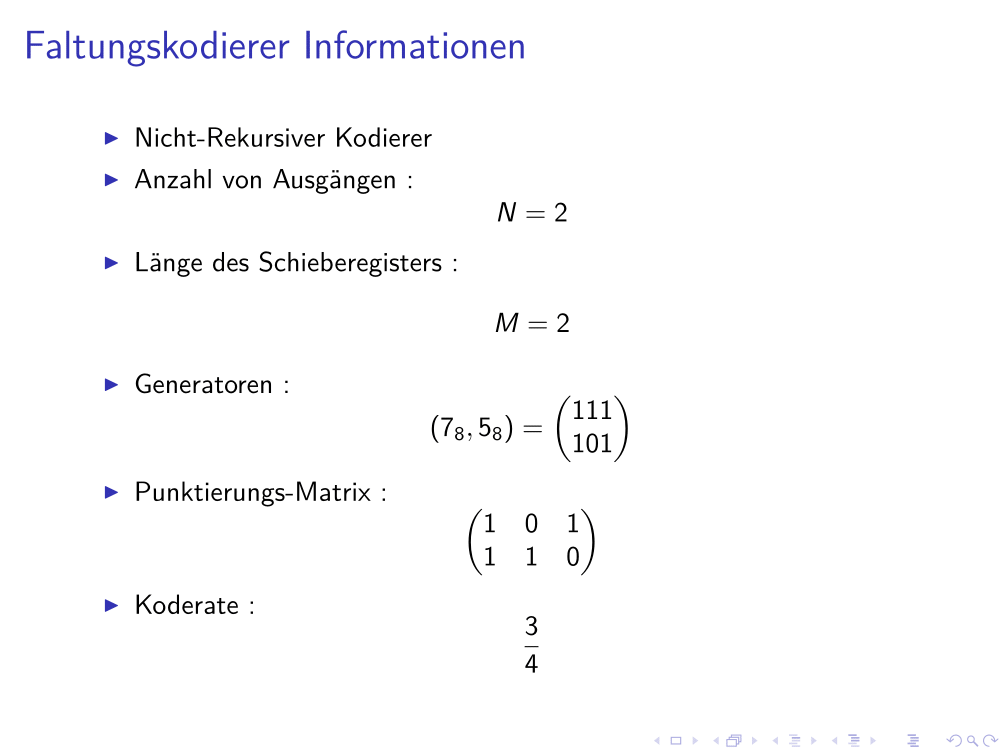
\includegraphics[width=0.99\textwidth]{abbildungen/folie_kodierung_info}}
		\caption{Folie mit Kodierer-Kennwerten}
		\label{abb:folie_kodierer_kennwerte}
	\end{subfigure}
	\quad % spacing between subfigures
	\begin{subfigure}{0.48\textwidth}
		\centering
		\fbox{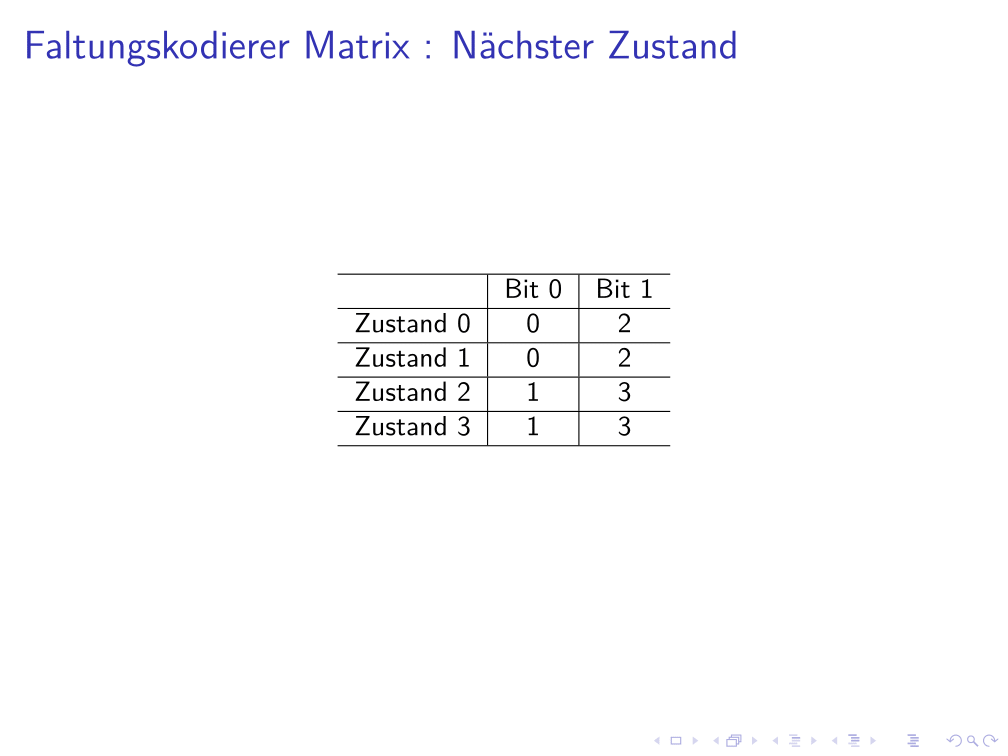
\includegraphics[width=0.99\textwidth]{abbildungen/folie_kodierung_matrix_zustand}}
		\caption{Folie mit Zustandsübergangsmatrix}
		\label{abb:folie_zustandsübergangsmatrix}
	\end{subfigure}
	\caption{Folien mit allgemeinen Informationen zum Faltungskodierer}
	\label{abb:folie_allg_info_kodierer}
\end{figure}
% Kodierung
Anschließend folgt die Visualisierung der Kodierung. Dabei wird die zu kodierende Nachricht Bit für Bit auf einer eigenen Folie verarbeitet. Abbildung~\ref{abb:folie_kodierung} zeigt die ersten beiden Schritte sowie den letzten Schritt der Kodierung. In Abbildung~\ref{abb:folie_kodierung_1} ist die Folie vor der Kodierung des ersten Bits zu sehen. Zunächst ist die zu kodierende Nachricht (Input), das Zustandsübergangsdiagramm, sowie eine noch nicht befüllte Kodierungstabelle zu sehen. Das Kodewort wird auf den folgenden Folien Schritt für Schritt erarbeitet. Durch diese Herangehensweise ist die Kodierung für den Benutzer einfach nachzuvollziehen. Abbildung~\ref{abb:folie_kodierung_2} zeigt die Folie der Kodierung des ersten Bits. Das erste Bit des Inputs, der aktuelle Zustand, der Folgezustand sowie der resultierende Output werden in eine neue Zeile der Kodierungstabelle geschrieben. Der aktuelle Zustand sowie der entsprechende Übergang werden im Diagramm farblich hervorgehoben, um die Kodierung auch im Zustandsdiagramm verfolgen zu können. Der Output wird auch unterhalb der Tabelle eingetragen und wächst mit jedem Schritt bis schlussendlich die gesamte Nachricht kodiert wurde. Die Visualisierung am Ende der Kodierung ist in Abbildung~\ref{abb:folie_kodierung_3} zu sehen. Die Bits unterhalb der horizontalen Trennlinie in der Tabelle stellen die Terminierungsbits dar.
\begin{figure}[th]
	\centering
	\begin{subfigure}{0.48\textwidth}
		\centering
		\fbox{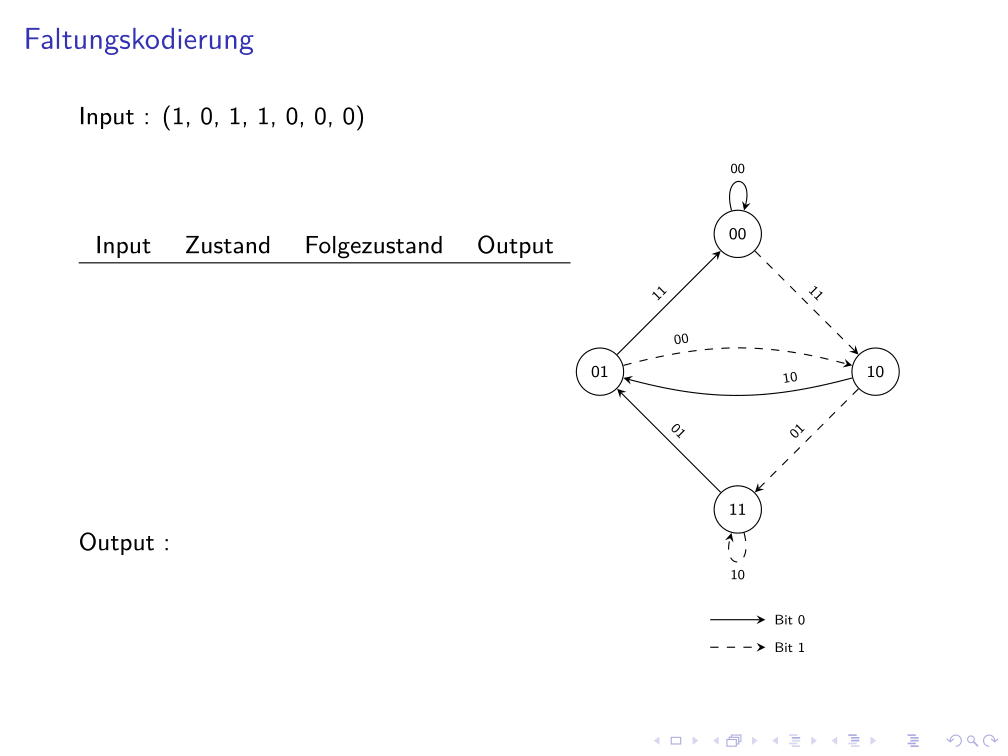
\includegraphics[width=0.99\textwidth]{abbildungen/folie_kodierung_1}}
		\caption{}
		\label{abb:folie_kodierung_1}
	\end{subfigure}
	\quad
	\begin{subfigure}{0.48\textwidth}
		\centering
		\fbox{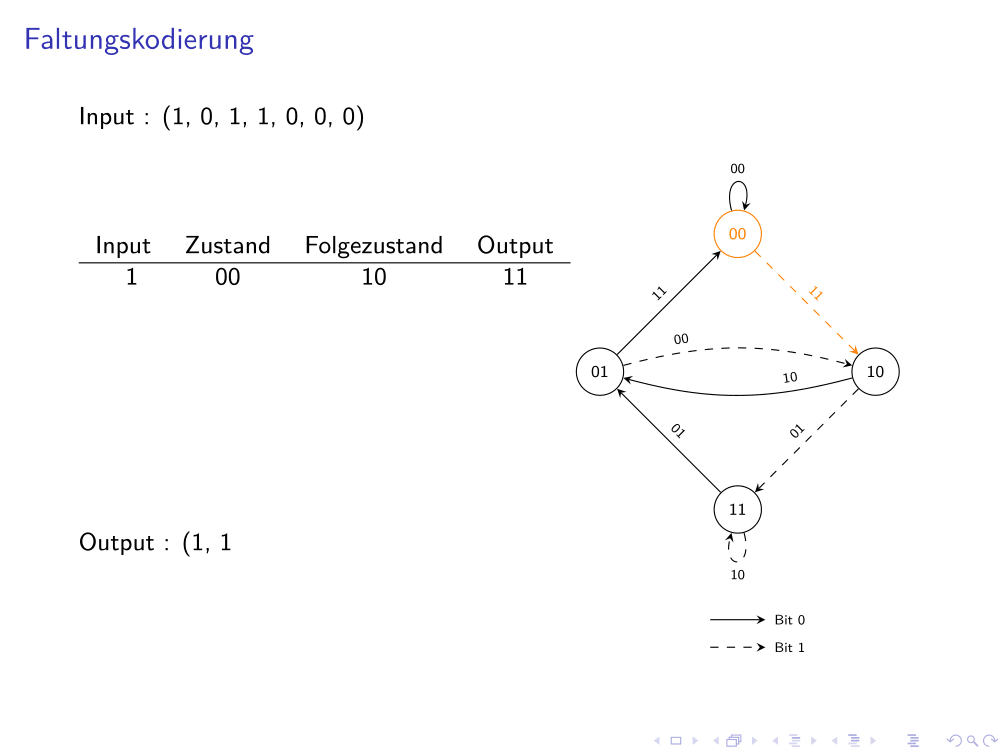
\includegraphics[width=0.99\textwidth]{abbildungen/folie_kodierung_2}}
		\caption{}
		\label{abb:folie_kodierung_2}
	\end{subfigure}
	\par\bigskip
	\begin{subfigure}{0.7\textwidth}
		\centering
		\fbox{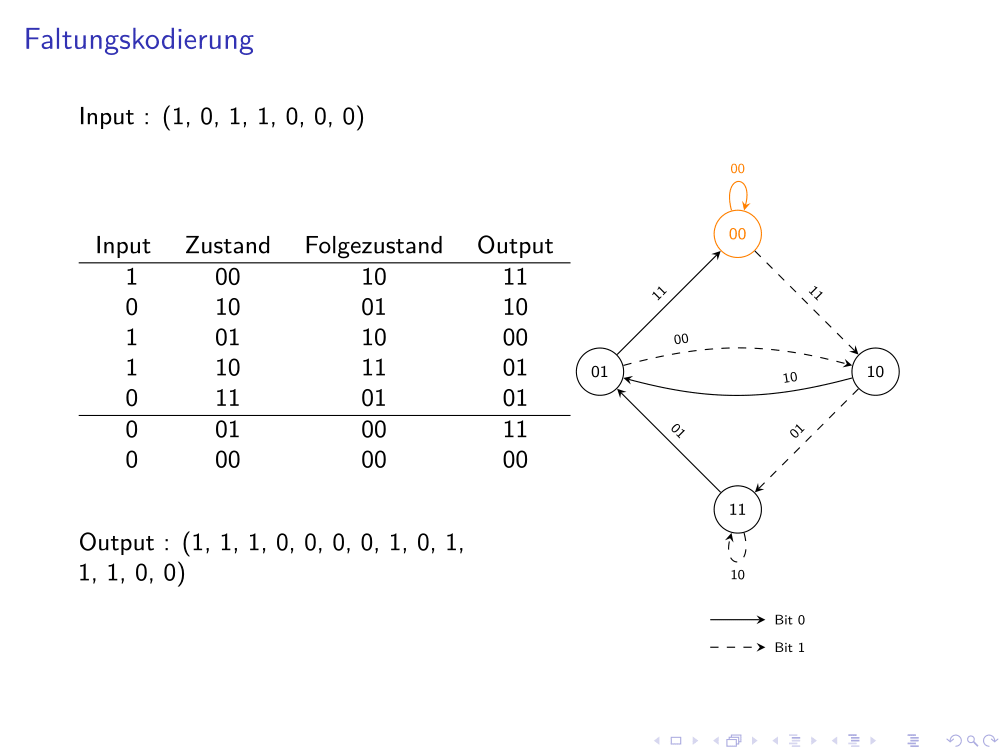
\includegraphics[width=0.99\textwidth]{abbildungen/folie_kodierung_3}}
		\caption{}
		\label{abb:folie_kodierung_3}
	\end{subfigure}
	\caption{Folien der Kodierung}
	\label{abb:folie_kodierung}
\end{figure}
% Kode zu Signal
Da die Kodierungsfunktion nicht die Bitwerte des Kodeworts zurückliefert, sondern die Signalwerte (für eine Übertragung über einen Kanal) wird auf einer weiteren Folie, wie in Abbildung~\ref{abb:folie_bit_zu_signal_abbildung} zu sehen, die Abbildung der Kodebits zu den Signalpegeln nach Gleichung~\eqref{eq:bit_zu_signal_abbildung} dargestellt.
\begin{figure}[th]
	\centering
	\fbox{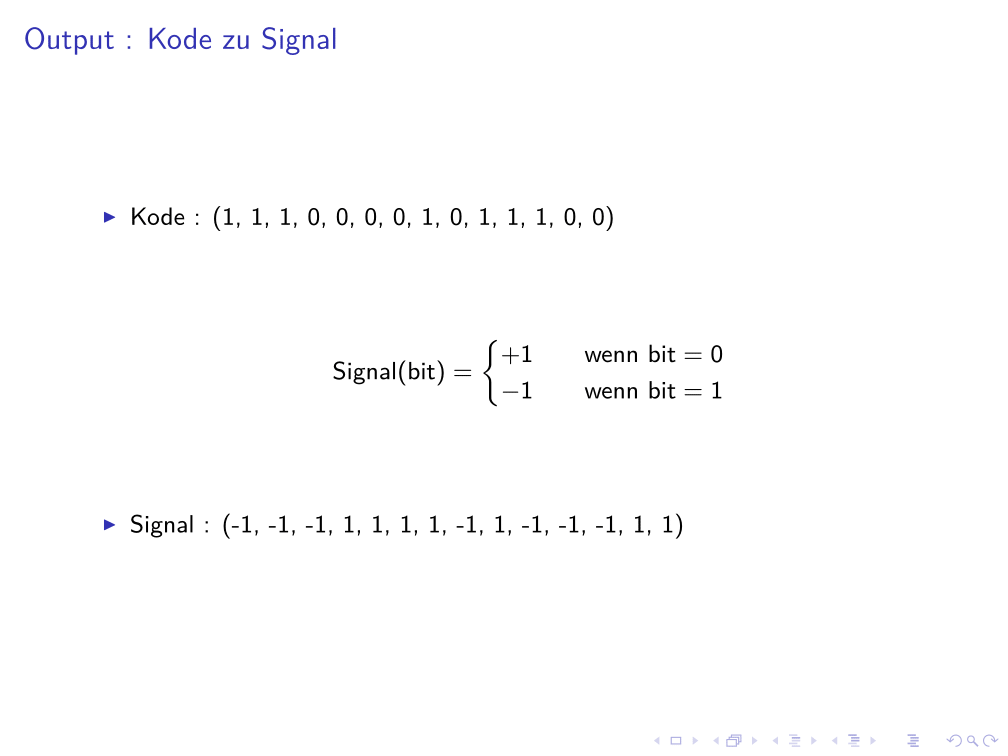
\includegraphics[width=0.7\textwidth]{abbildungen/folie_kodierung_bit_zu_signal}}
	\caption{Folie mit der Abbildung der Kodebits zu den Signalpegeln}
	\label{abb:folie_bit_zu_signal_abbildung}
\end{figure}
% Punktierung
Abbildung~\ref{abb:folie_punktierung} zeigt die Folie der Punktierung. Auf dieser wird die Punktierung des Signals, d.h. das Entfernen von Signalwerten (definiert durch die Punktierungsmatrix) dargestellt. Dabei wird, neben dem originalen Signal und der Punktierungsmatrix, das punktierte Signal dargestellt, wobei zunächst die punktierten Signalwerte, d.h. die entfernten Werte, durch Asterisk-Symbole ($\ast$) ersetzt werden. Diese Darstellung dient als visueller Zwischenschritt für das anschließende tatsächlich punktierte Signal, bei dem die punktierten Werte fehlen, was dem Rückgabewert der Funktion entspricht.
\begin{figure}[th]
	\centering
	\fbox{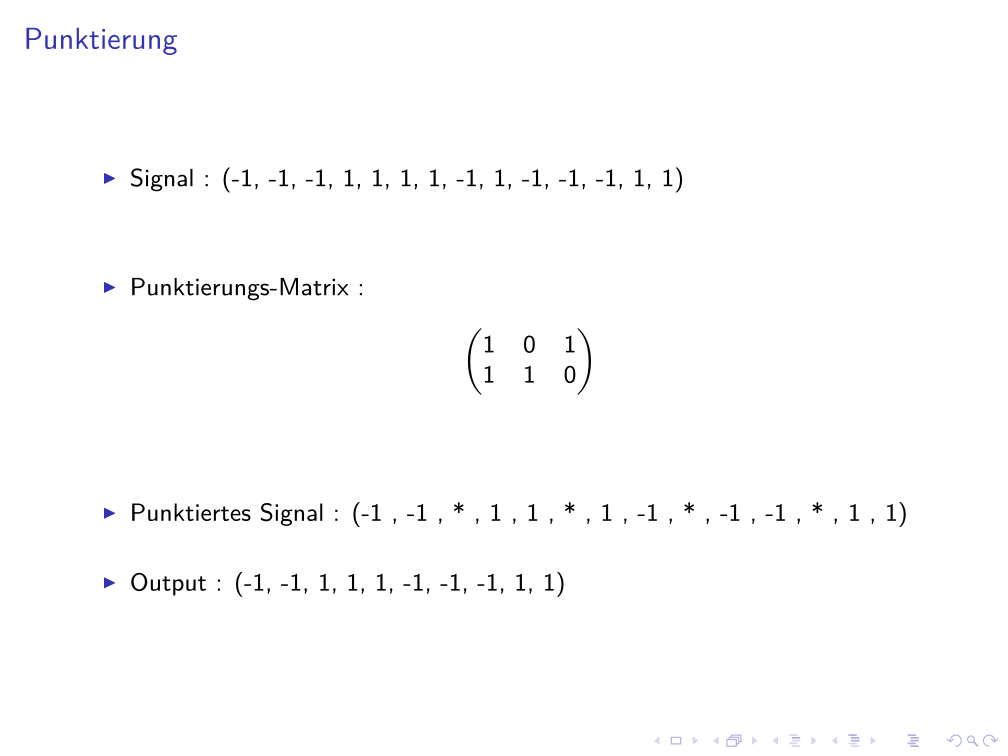
\includegraphics[width=0.7\textwidth]{abbildungen/folie_kodierung_punktierung}}
	\caption{Folie mit Punktierung}
	\label{abb:folie_punktierung}
\end{figure}
\FloatBarrier
\section{Dekodierung}
\label{kapitel:visualisierung_dekodierung}
% allg. Informationen
Bei der Dekodierung befinden sich ebenfalls, wie bei der Kodierung, allgemeine Informationen des Faltungskodierers auf den ersten Folien.
\\
% Depunktierung
Abbildung~\ref{abb:folie_depunktierung} zeigt die Folie der Depunktierung. Auf dieser wird die Depunktierung des Signals, d.h. das Einfügen des Signalwerts 0 (definiert durch die Punktierungsmatrix), dargestellt. Die eingefügten 0-Werte sind zur leichteren visuellen Erkennung farblich hervorgehoben.
\begin{figure}[th]
	\centering
	\fbox{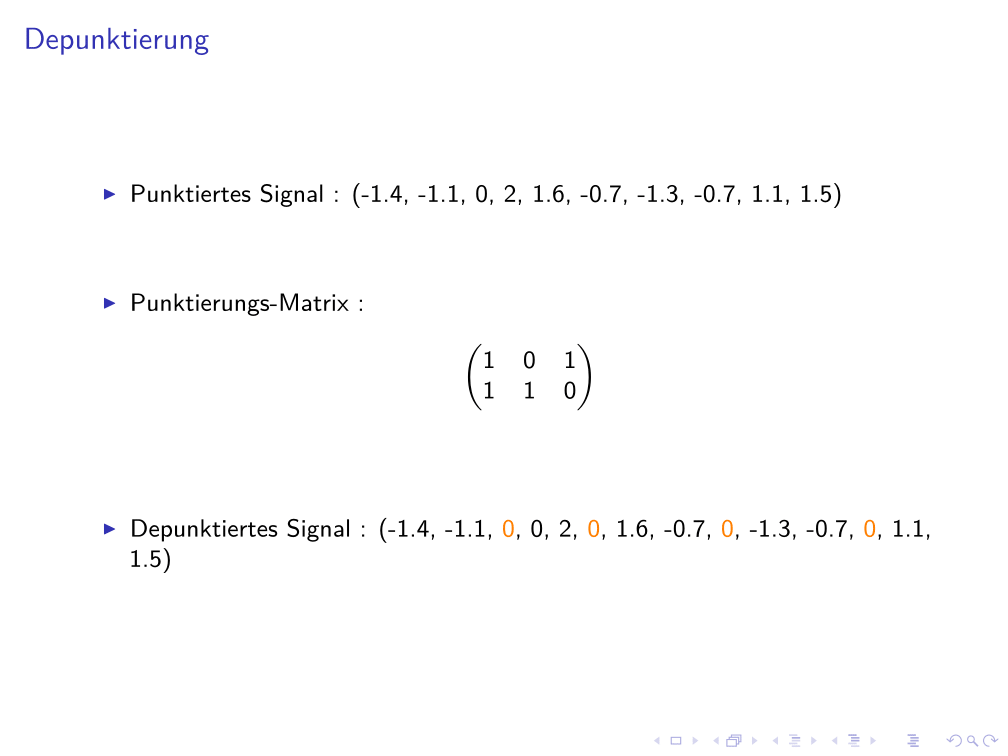
\includegraphics[width=0.7\textwidth]{abbildungen/folie_dekodierung_depunktierung}}
	\caption{Folie mit Depunktierung}
	\label{abb:folie_depunktierung}
\end{figure}
% Signal zu Kode
Als Input erhält die Dekodierung das Kodewort als kontinuierliche Signalwerte, die möglicherweise durch Anwendung der \texttt{ApplyNoise}-Funktion verfälscht worden sind. Die soft decision Dekodierung verwendet zur Dekodierung zwar direkt diese Signalwerte, da aber sowohl die hard decision Dekodierung Bitwerte zur Dekodierung verwendet, als auch die Kanten des Trellis mit Bitwerten beschriftet sind, wird der Input, um konsistent zu bleiben, auf Bitwerte abgebildet. Die Folie der Abbildung der Signalwerte auf Bitwerte (nach Gleichung~\ref{eq:signal_zu_bit_abbildung}) ist in Abbildung~\ref{abb:folie_signal_zu_bit_abbildung} zu sehen.
\begin{figure}[th]
	\centering
	\fbox{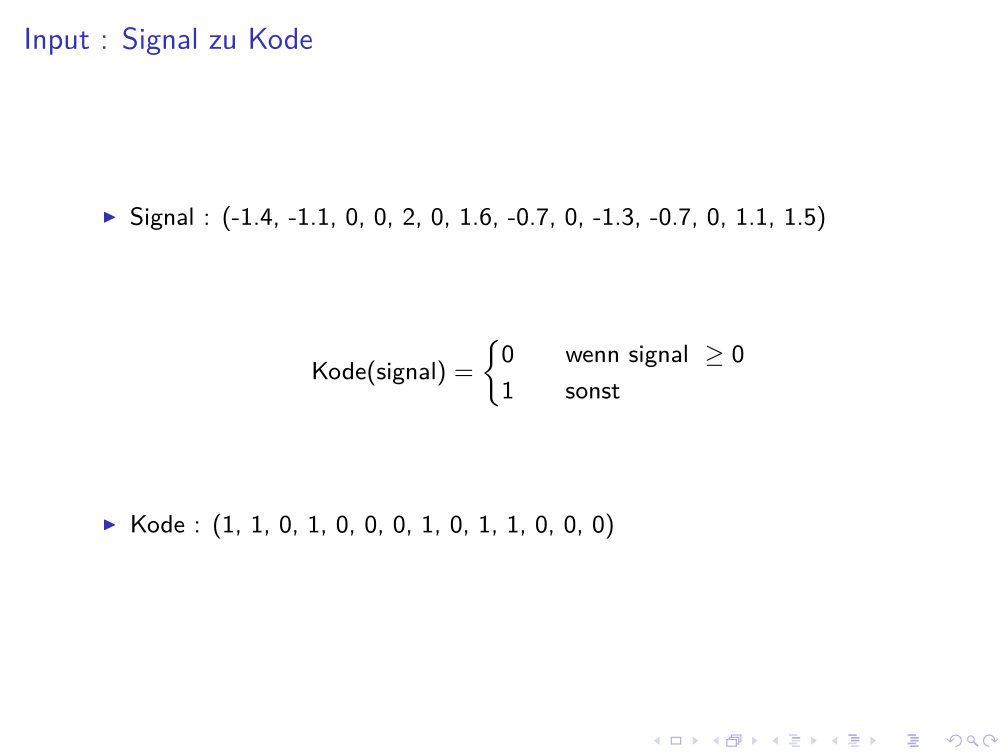
\includegraphics[width=0.7\textwidth]{abbildungen/folie_dekodierung_signal_zu_bit}}
	\caption{Folie mit der Abbildung der Signalpegel zu den Kodebits}
	\label{abb:folie_signal_zu_bit_abbildung}
\end{figure}
% Viterbi-Algorithmus
Anschließend folgt die Visualisierung des Viterbi-Algorithmus mithilfe des Trellis-Diagramms. In den farbigen Kreisen befinden sich die Metriken der Pfade, die zum jeweiligen Zustand führen. Zunächst werden, zur besseren Übersicht bei großen Diagrammen, jene Pfade entfernt, für die es eine bessere Alternative gibt. D.h. es werden jene Pfade entfernt die bei der soft decision Dekodierung eine niedrigere Metrik bzw. bei der hard decision Dekodierung eine höhere Metrik besitzen. Dieser Schritt ist zwischen den Abbildungen~\ref{abb:folie_dekodierung_1} und \ref{abb:folie_dekodierung_2} zu sehen. Danach erfolgt Schritt für Schritt die Rekonstruktion der Nachricht mittels Backtracking. Der gewählte Pfad beim Backtracking wird farblich hervorgehoben. Die übrigen Pfade werden ausgegraut. Eine Folie während des Backtrackings wird in Abbildung~\ref{abb:folie_dekodierung_3} veranschaulicht. Am Ende befindet sich unter dem Trellis-Diagramm die farblich hervorgehobene dekodierte Nachricht, wie in Abbildung~\ref{abb:folie_dekodierung_4} dargestellt. Die einzelnen Zwischenschritte vermitteln dem Benutzer wie der Algorithmus funktioniert und wie sich die dekodierte Nachricht ergibt.
\begin{figure}[th]
	\centering
	\fbox{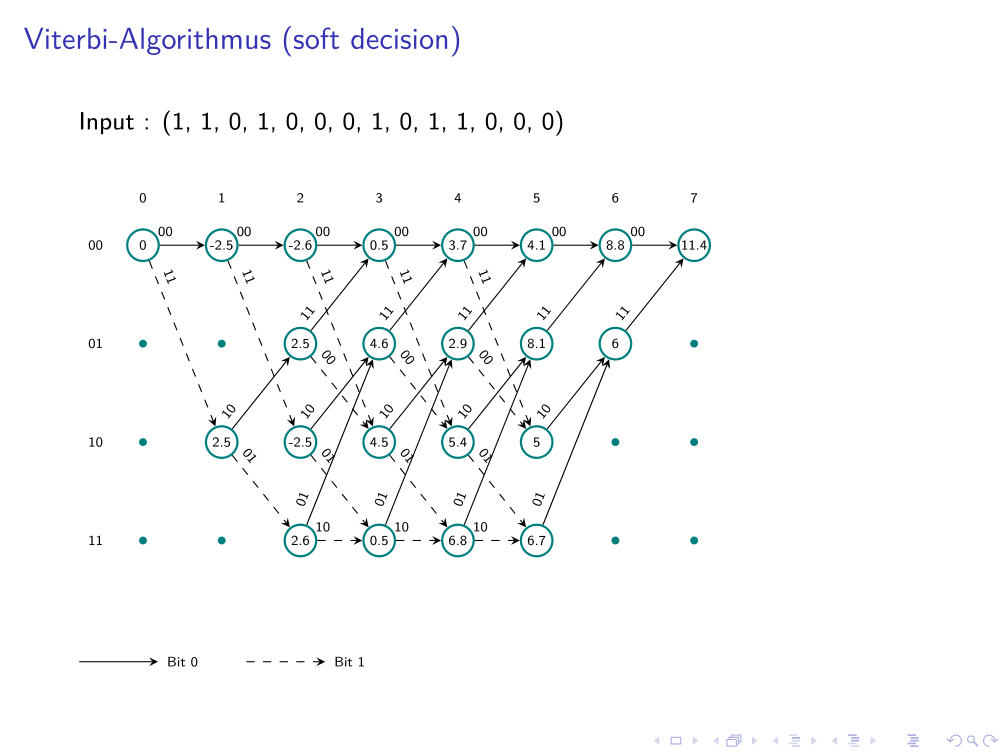
\includegraphics[width=0.7\textwidth]{abbildungen/folie_dekodierung_1}}
	\caption{Folie der soft decision Dekodierung und dem vollständigen Trellis}
	\label{abb:folie_dekodierung_1}
\end{figure}
\begin{figure}[th]
	\centering
	\fbox{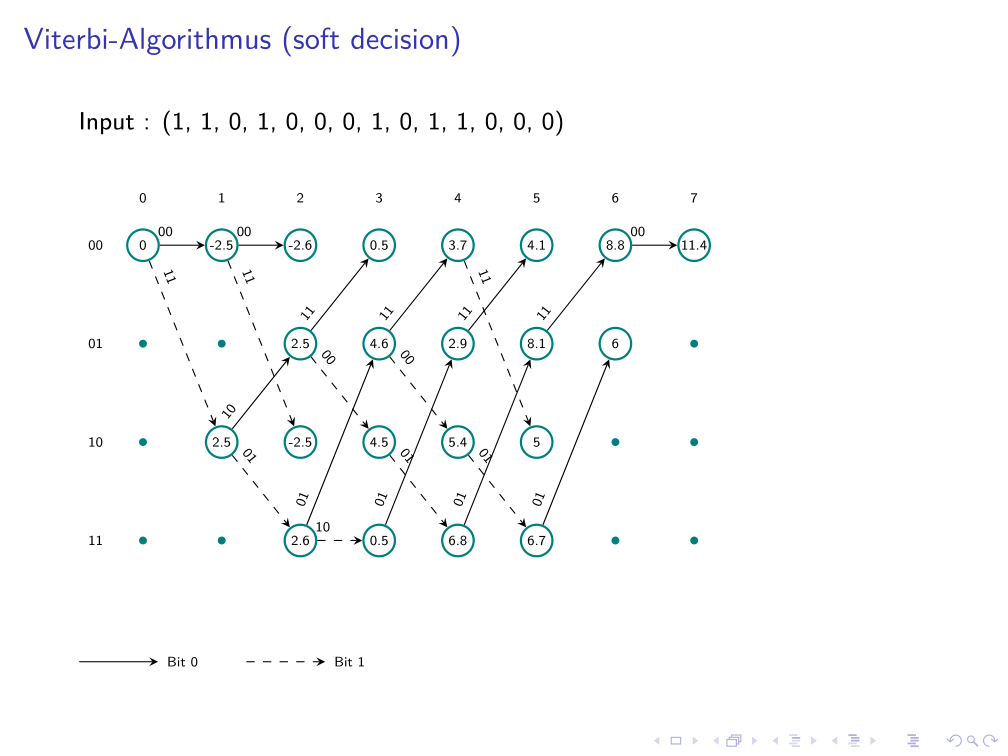
\includegraphics[width=0.7\textwidth]{abbildungen/folie_dekodierung_2}}
	\caption{Folie der soft decision Dekodierung und dem Trellis nach dem Entfernen einiger Pfade}
	\label{abb:folie_dekodierung_2}
\end{figure}
\begin{figure}[th]
	\centering
	\fbox{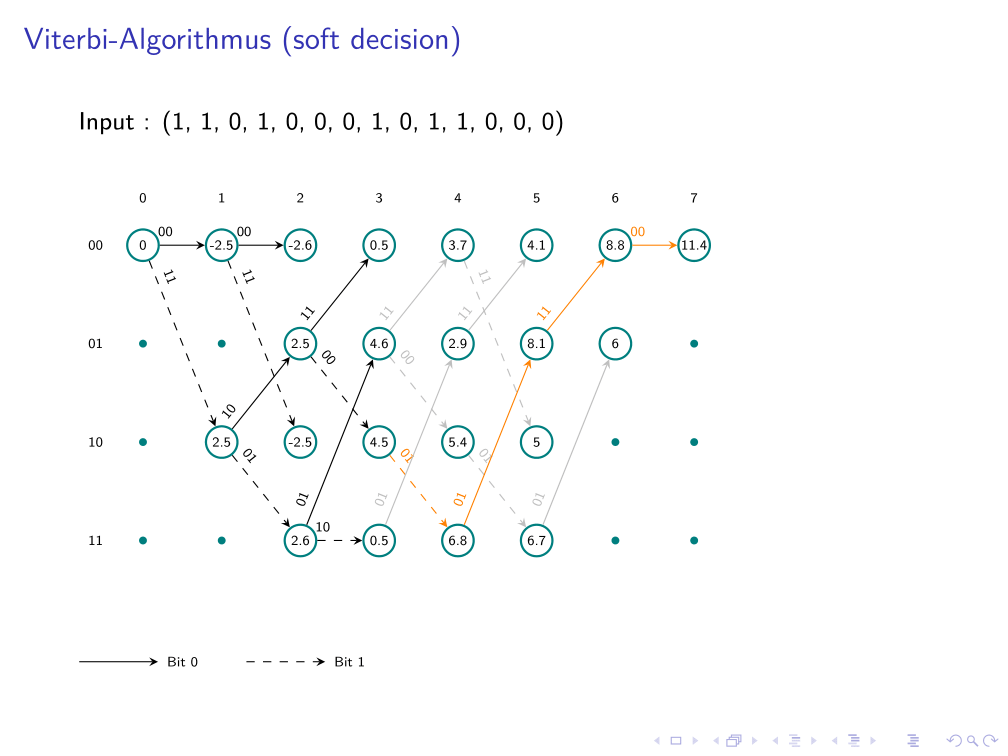
\includegraphics[width=0.7\textwidth]{abbildungen/folie_dekodierung_3}}
	\caption{Folie der soft decision Dekodierung im während dem Backtracking}
	\label{abb:folie_dekodierung_3}
\end{figure}
\begin{figure}[th]
	\centering
	\fbox{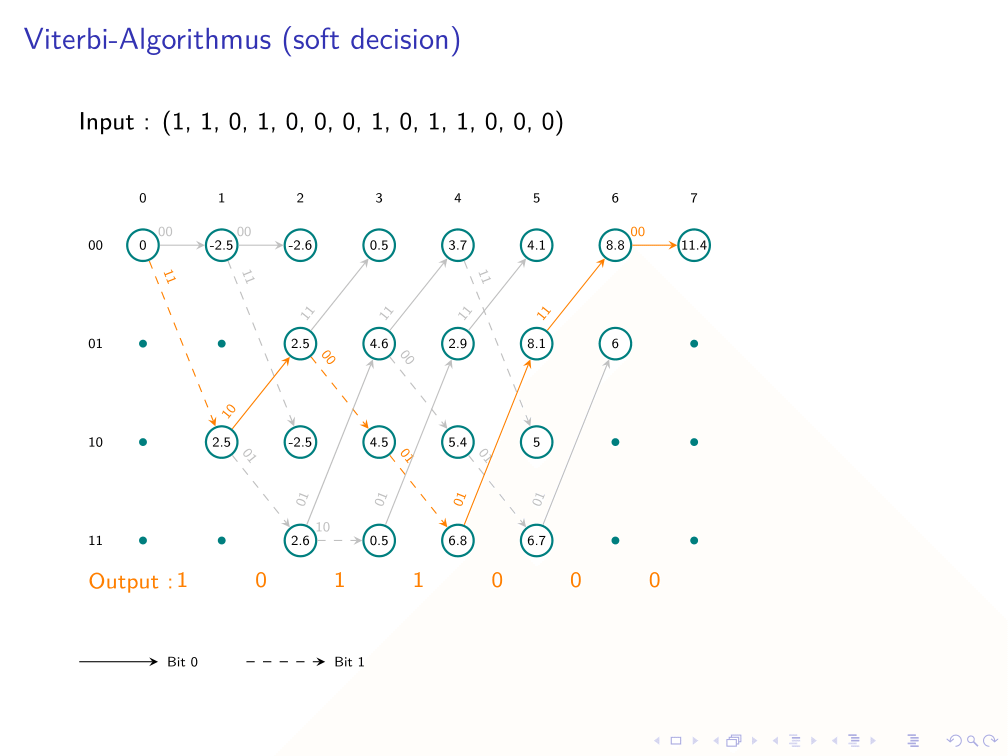
\includegraphics[width=0.7\textwidth]{abbildungen/folie_dekodierung_4}}
	\caption{Folie der soft decision Dekodierung mit der dekodierten Nachricht}
	\label{abb:folie_dekodierung_4}
\end{figure}

\section{Simulation}
\label{kapitel:visualisierung_simulation}
Auch die Simulationsfunktionen bieten durch den \texttt{visualize}-Parameter die Möglichkeit eine Visualisierung generieren zu lassen. Kapitel~\ref{kapitel:visualisierung_simulation_faltungskodierung} erläutert die Präsentation der Faltungskode-Simulation. Die Folien der Simulation verschiedener Varianten der Kanalkodierung, um diese vergleichen zu können, sind in Kapitel~\ref{kapitel:visualisierung_simulation_kanalkodierung} beschrieben.

\subsection{Faltungskodierung}
\label{kapitel:visualisierung_simulation_faltungskodierung}
Die folgenden Folien sind das Resultat der Ausführung der \texttt{ConvSimulation}-Funktion. Auf den ersten Folien sind, wie schon bei der Kodierung und Dekodierung, Informationen zum verwendeten Faltungskodierer angegeben.
\\
Anschließend folgt eine Folie mit den Eckdaten der Simulation, wie in Abbildung~\ref{abb:folie_simulation_f1} ersichtlich.
\\
Die nächste Folie, dargestellt in Abbildung~\ref{abb:folie_simulation_f2}, stellt ein Diagramm der Daten des erzeugten Dataframes dar. Die x-Achse entspricht dem Signal-Rausch-Verhältnis. Auf der y-Achse werden die gemessenen Bitfehlerraten aufgetragen. Es ist in diesem Beispiel sehr gut zu erkennen, dass die Fehleranzahl mit steigendem Signal-Rausch-Verhältnis abnimmt.
\\
Abschließend werden statistische Kennzahlen der Bitfehlerraten wie Minimum, Maximum, Median etc. auf der letzten Folie, wie in Abbildung~\ref{abb:folie_simulation_f3} zu sehen, aufgelistet. 
\begin{figure}[th]
	\centering
	\begin{subfigure}{0.48\textwidth}
		\centering
		\fbox{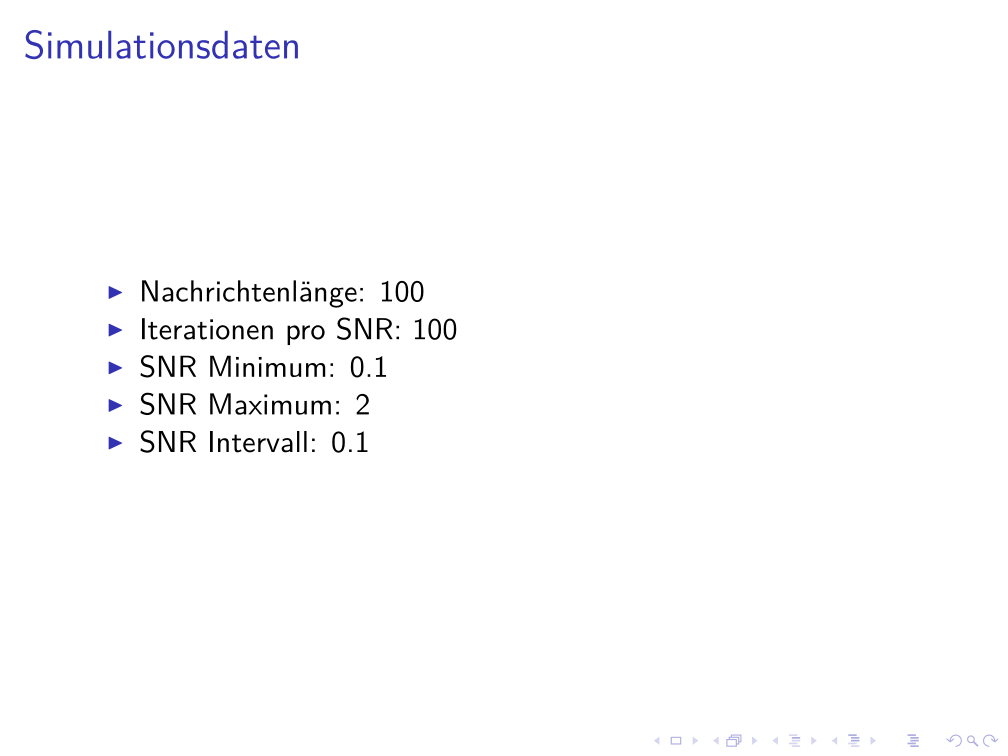
\includegraphics[width=0.99\textwidth]{abbildungen/folie_simulation_f1}}
		\caption{Folie mit Simulationseckdaten\\ \textcolor{white}{x}}
		\label{abb:folie_simulation_f1}
	\end{subfigure}
	\quad
	\begin{subfigure}{0.48\textwidth}
		\centering
		\fbox{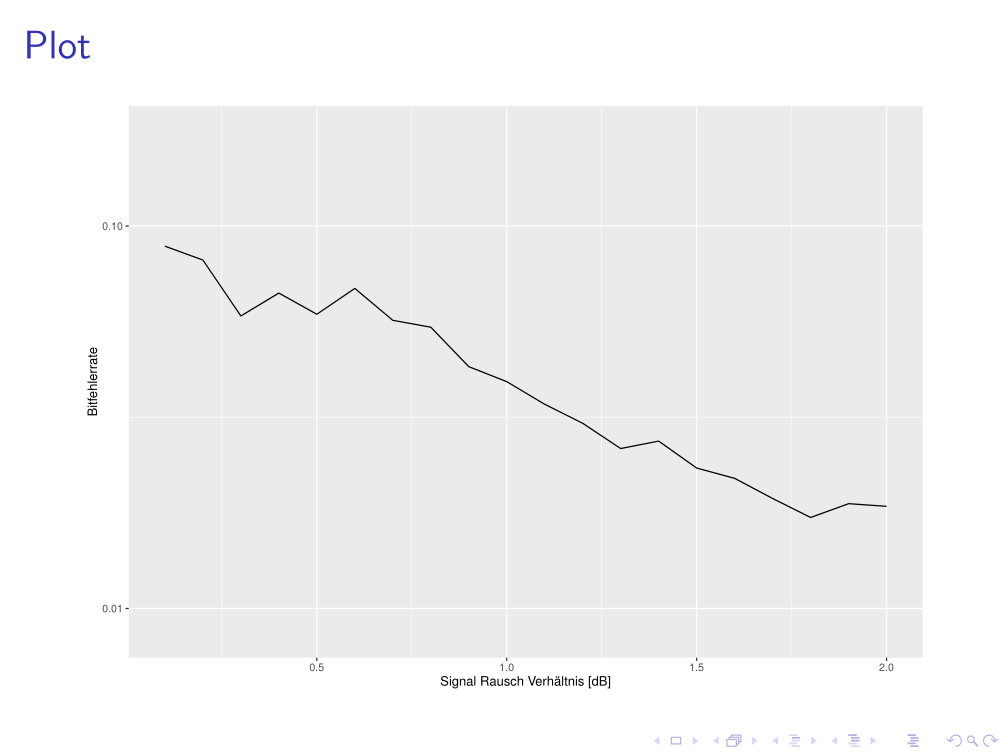
\includegraphics[width=0.99\textwidth]{abbildungen/folie_simulation_f2}}
		\caption{Folie mit Diagramm der Simulationsergebnisse}
		\label{abb:folie_simulation_f2}
	\end{subfigure}
	\par\bigskip
	\begin{subfigure}{0.48\textwidth}
		\centering
		\fbox{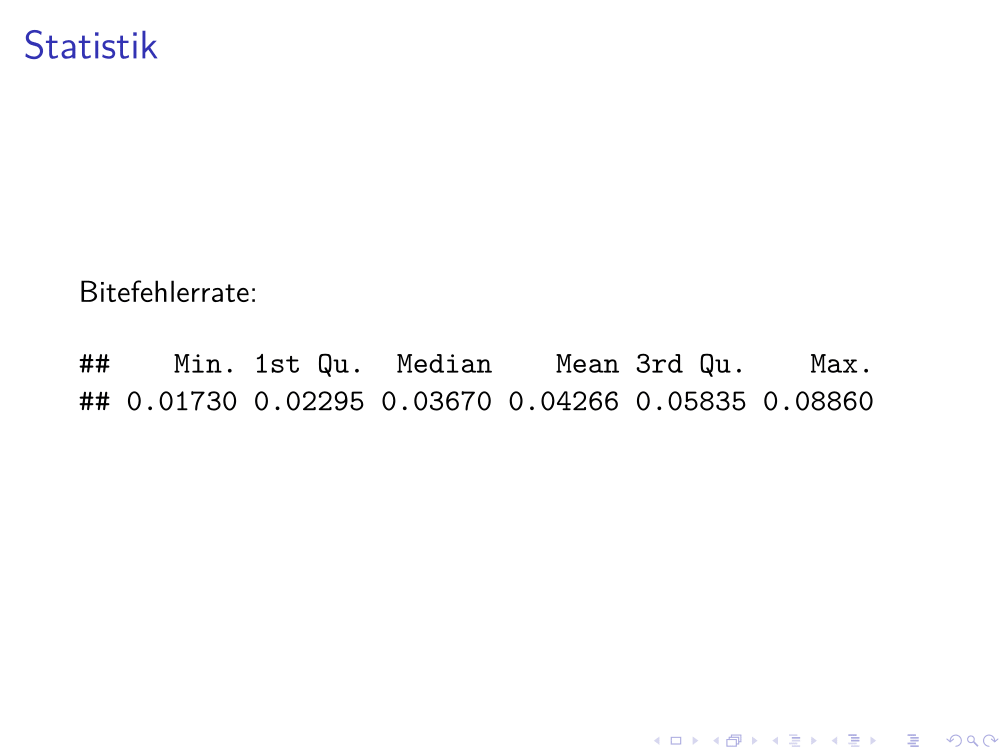
\includegraphics[width=0.99\textwidth]{abbildungen/folie_simulation_f3}}
		\caption{Folie mit Statistik der Bitfehlerraten}
		\label{abb:folie_simulation_f3}
	\end{subfigure}
	\caption{Folien der Faltungskodierungs-Simulation}
	\label{abb:folie_simulation_f}
\end{figure}

\subsection{Kanalkodierung}
\label{kapitel:visualisierung_simulation_kanalkodierung}
\begin{figure}[th]
	\centering
	\begin{subfigure}{0.48\textwidth}
		\centering
		\fbox{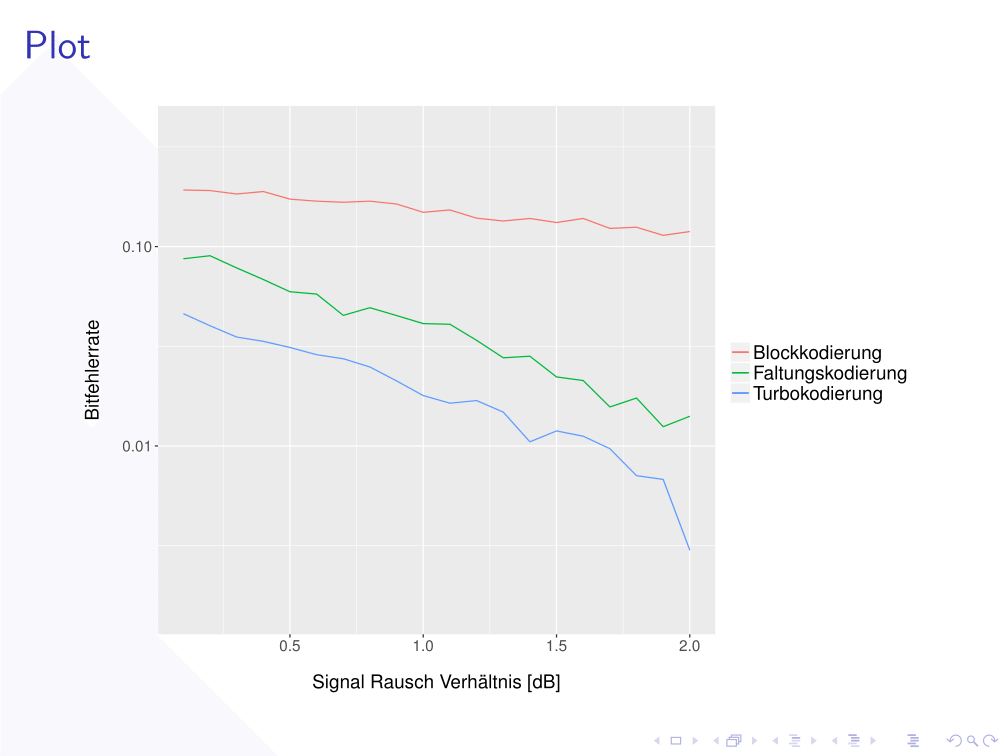
\includegraphics[width=0.99\textwidth]{abbildungen/folie_simulation_k1}}
		\caption{Folie mit Diagramm der Ergebnisse}
		\label{abb:folie_simulation_k1}
	\end{subfigure}
	\quad
	\begin{subfigure}{0.48\textwidth}
		\centering
		\fbox{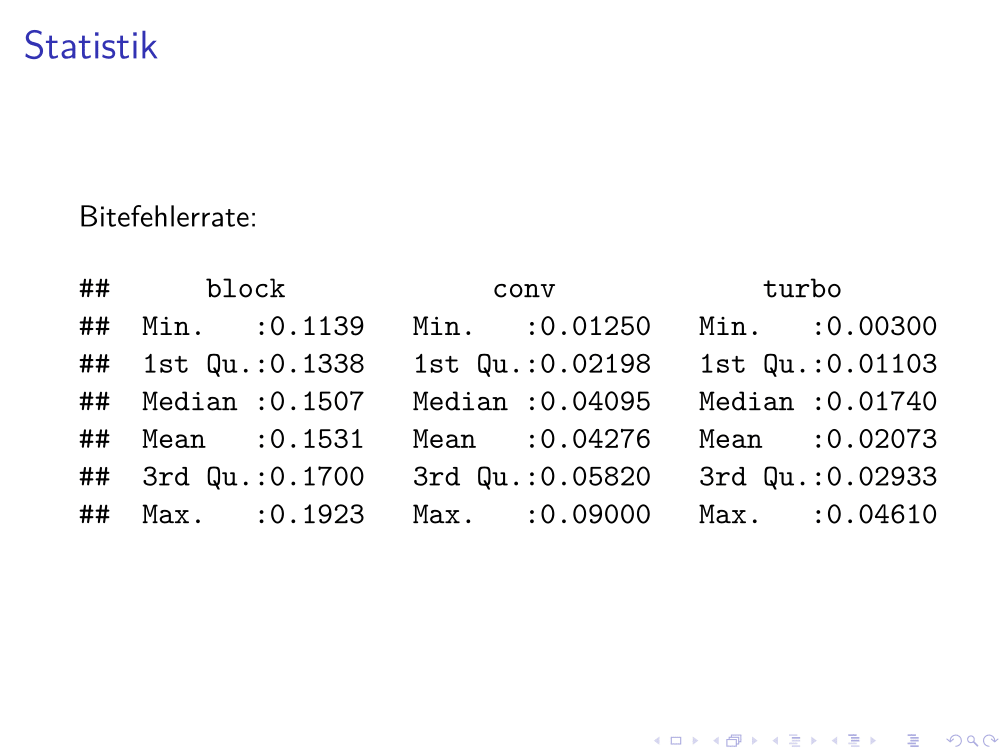
\includegraphics[width=0.99\textwidth]{abbildungen/folie_simulation_k2}}
		\caption{Folie mit Simulationsstatistik}
		\label{abb:folie_simulation_k2}
	\end{subfigure}
	\caption{Folien der Kanalkodierungs-Simulation}
	\label{abb:folie_simulation_k}
\end{figure}
Für einen Vergleich der im R-Paket implementierten Verfahren der Kanalkodierung kann die \texttt{ChannelcodingSimulation}-Funktion ausgeführt werden, deren Simulationsergebnisse ebenfalls dargestellt werden können. Zu Beginn der Kanalkodierungs-Visualisierungen werden auf einer Folie die Simulationseckdaten aufgelistet, wie es schon bei der Visualisierung der Faltungskodierungs-Simulation der Fall war.
\\
Abbildung~\ref{abb:folie_simulation_k1} zeigt die Folie mit dem Diagramm, in dem die Ergebnisse der drei Simulationen dargestellt werden und miteinander verglichen werden können. Die Art der Kodierung einer Kurve kann anhand der Farbe zugeordnet werden.
%\begin{figure}[th]
%	\centering
%	\fbox{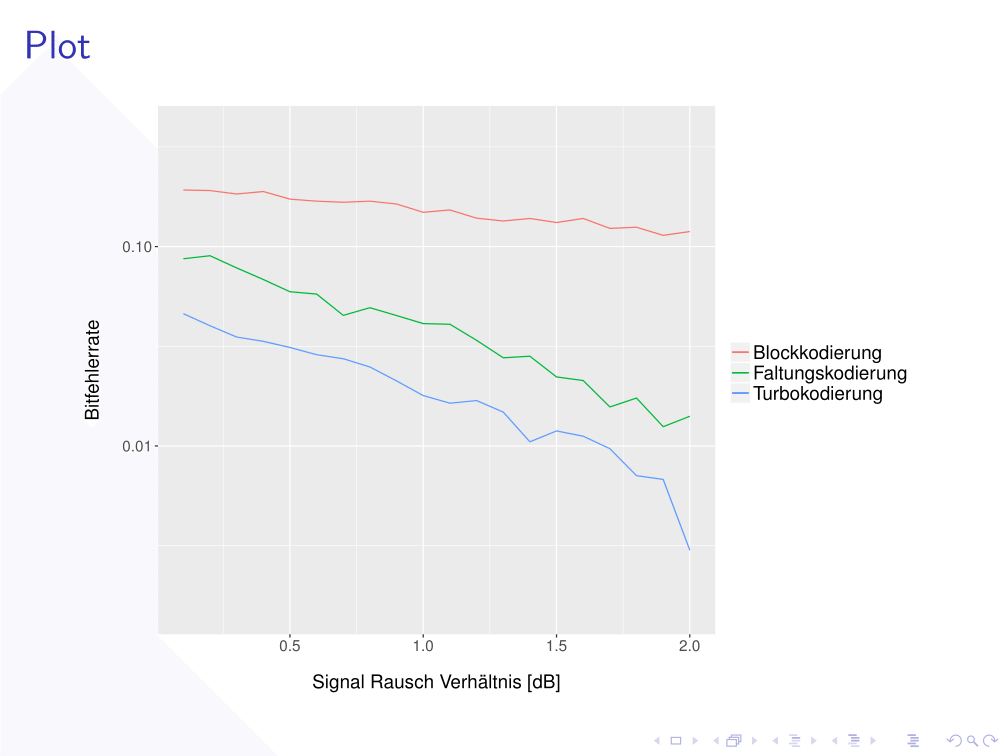
\includegraphics[width=0.7\textwidth]{abbildungen/folie_simulation_k1}}
%	\caption{Folie mit Diagramm der Ergebnisse der Kanalkodierungs-Simulationen}
%	\label{abb:folie_simulation_k1}
%\end{figure}
Wie auch schon in Kapitel~\ref{kapitel:visualisierung_simulation_faltungskodierung} befindet sich auf der letzten Folie eine Statistik der Bitfehlerraten. Dabei werden die Werte der verschiedenen Kanalkodierungs-Varianten gegenübergestellt. Abbildung~\ref{abb:folie_simulation_k2} zeigt ein Beispiel zur Statistik-Folie.
%\begin{figure}[th]
%	\centering
%	\fbox{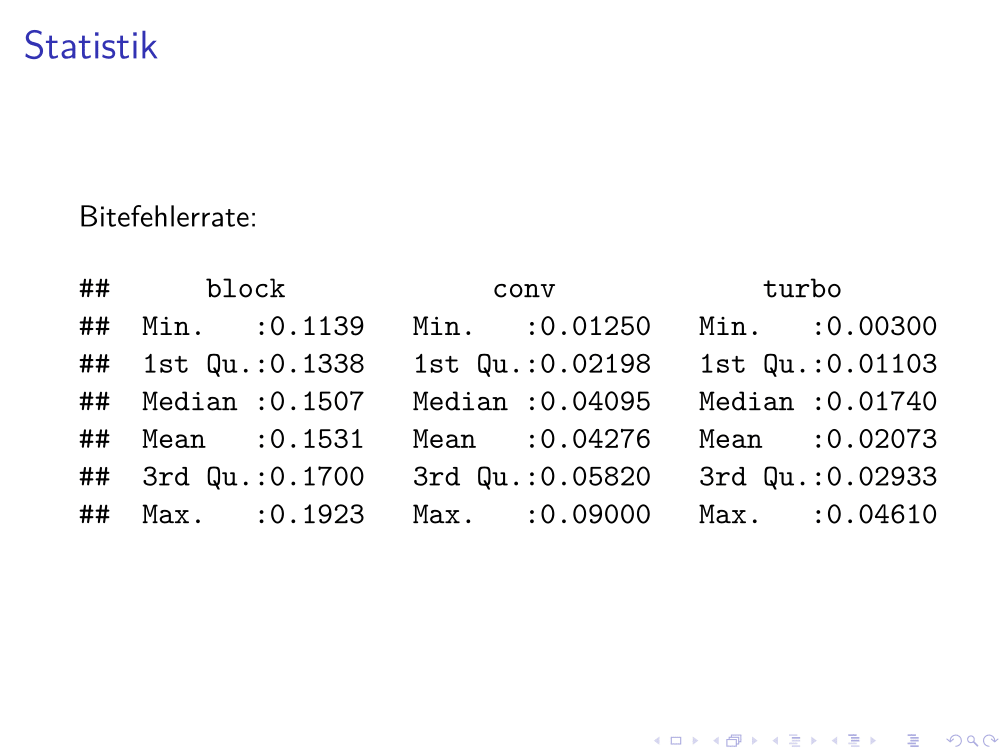
\includegraphics[width=0.7\textwidth]{abbildungen/folie_simulation_k2}}
%	\caption{Folie mit Simulationsstatistik}
%	\label{abb:folie_simulation_k2}
%\end{figure}

\chapter{Beispiele für die Verwendung}
\label{chapter:examples}
Um dem Benutzer den Einstieg zur Verwendung des Paketes zu erleichtern, sind in den folgenden Kapiteln Beispiele und genaue Erklärungen zu allen wichtigen Funktionen. Dabei wird im Kapitel \ref{sec:example_createHelpers} alle wichtigen Variablen erstellt, die dann in den Kapiteln \ref{sec:example_withPunctuation} und \ref{sec:example_withoutPunctuation} beim Kodieren und Dekodieren verwendet werden. Zum Schluss wird im Kapitel \ref{sec:example_simulations} die verschiedenen Möglichkeiten der Ausführung von Simulationen erläutert.

\section{Erzeugen von Kodierer, Permutationsvektor und Punktierungsmatrix}
\label{sec:example_createHelpers}
Zuerst werden Hilfsvariablen erzeugt, die für die folgende Kodierungs- und Dekodierungsverfahren benötigt werden. Diese Variablen müssen nicht unbedingt mitgegebenen werden, dann werden die Standard-Werte verwendet. Das bedeutet, dass falls keine Punktierungsmatrix übergeben wird, der Standard-Wert \emph{NULL} ist und darum nicht punktiert wird. Ebenfalls wird nicht permutiert, wenn kein Permutationsvektor als Argument übergeben wird. Es wird zwar ein Permutationsvektor benötigt, damit die Interleaver richtig arbeiten können, jedoch wird ein Vektor vom Typ \emph{PRIMITIVE} verwendet, dieser allerdings ändert die Reihenfolge der Bits nicht (root=0). Beim Kodierer verhält es sich ähnlich, jedoch wird hier ein vordefinierter Standard-Faltungskodierer verwendet (\emph{ConvGenerateRscEncoder(2,2,c(5,7))}), dieser wird in allen Turbo-Kode-Funktionen benützt, falls kein eigener Kodierer übergeben wird.

\begin{lstlisting}[caption=Erzeugung von Kodierer und Punktierungsmatrix, label={lst:createHelpersCoderPunctuation}, float=ht]
input <- c(1,0,1,1,0)

coder <- ConvGenerateEncoder(2, 2, c(4,5))

punctuation.matrix <- TurboGetPunctuationMatrix(c(1,1,0))
\end{lstlisting}

Wie im Listing \ref{lst:createHelpersCoderPunctuation} zu sehen ist, wird als allererstes eine zu kodierende Nachricht erzeugt, die dann benötigt wird, die dann benötigt wird um eine Punktierungsmatrix zu bekommen. Anschließend wird ein nicht rekursiver Faltungskodierer, mit der Funktion vom Faltungskode-Teil des Packetes \cite{nocker}, erzeugt. Dabei wurde ein Kodierer mit zwei Registern und zwei Ausgängen gewählt. Wichtig ist, dass der erste Ausgang vom Eingang durchgeschalten wird damit es ein systematischer Kodierer ist. Das wird erreicht, indem das erste Generatorpolynom mit $2^M = 2^2 = 4$ deklariert wird. Zum Schluss wird noch eine Punktierungsmatrix erstellt, die aus nur einer Spalte besteht und jedes dritte Bit aus dem Vektor entfernt. Bei einer 1 wird das Bit behalten, bei einer 0 verworfen.

\begin{lstlisting}[caption=Erzeugung von verschiedenen Permutationsvektoren, label={lst:createHelpersPermutation}, float=ht]
permutation.vector.random <- TurboGetPermutation(length(input), coder, "RANDOM")
permutation.vector.primitve <- TurboGetPermutation(length(input), coder, "PRIMITIVE", list(root=3))

input2 <- c(1,0,1,1,0,1)
permutation.vector.cyclic <- TurboGetPermutation(length(input2), coder, "CYCLIC", list(cols=4, rows=2, distance=2))
permutation.vector.block <- TurboGetPermutation(length(input2), coder, "BLOCK", list(cols=4, rows=2))
permutation.vector.helical <- TurboGetPermutation(length(input2), coder, "HELICAL", list(cols=4, rows=2))
permutation.vector.diagonal <- TurboGetPermutation(length(input2), coder, "DIAGONAL", list(cols=4, rows=2))
\end{lstlisting}

Als nächstes benötigt der Benutzer noch einen Permutationsvektor, dieser wird im Listing \ref{lst:createHelpersPermutation} erzeugt. Dabei wird jeder Typ einmal verwendet. Bei den ersten beiden werden die Eingangsbits von Listing \ref{lst:createHelpersCoderPunctuation} benützt. Da bei den restlichen Typen eine Matrix benötigt wird, muss die Länge der Eingangsbits genau in einer Matrix Platz finden, deshalb wurde ein zweiter Eingangsvektor definiert, der allerdings nur als Demonstration für die anderen Permutationstypen dienen sollte, dieser wird in den weiteren Beispielen nicht weiter verwendet.

\section{Kodieren und Dekodieren ohne Punktierung}
\label{sec:example_withoutPunctuation}
Nachdem alle benötigten Variablen gesetzt wurden kann nun die Kodierung und Dekodierung vorgenommen werden. Dabei wird zuerst ohne Punktierung gearbeitet, jedoch alle anderen zuvor definierten Variablen verwendet.

\begin{lstlisting}[caption=Kodierung und Dekodierung ohne Punktierung, label={lst:encodeDecodeWithoutPunctuation}, float=ht]
encoded <- TurboEncode(input, permutation.vector.random, coder, 2)
encoded
[1] -1 -1 -1  1  1  1 -1  1  1 -1 -1  1  1 -1 -1  1 -1 -1  1  1  1

encoded.noisy <- ApplyNoise(encoded, 0.1)
round(encoded.noisy, 2)
[1] -2.41 -2.36 -0.26  1.06  1.37  0.22  1.13  0.93  0.33 -1.15 -1.18  0.59
[13]  1.32 -0.31 -1.37 -0.01 -1.42 -1.62  2.18  2.29  0.93

decoded <- TurboDecode(encoded.noisy, permutation.vector.random, 5, coder, 2)
decoded
$output.soft
[1]  -1.394185  1.394185  2.775904 -1.394185  2.775904

$output.hard
[1] 1 0 1 1 0
\end{lstlisting}

Der gesamte Vorgang lässt sich in wenigen Zeilen erledigen, wie in Listing \ref{lst:encodeDecodeWithoutPunctuation} zu sehen ist. Zuerst werden einfach die zuvor definierten Variablen der Kodierungsfunktion mitgegeben, als letzter Parameter wird noch der Index des zu verwendeten Ausgangs des Kodierers angegeben (zwei in diesem Fall). Danach erhält man das kodierte Signal mit dem Signalpegel 1 und -1. Dieses Signal wird dann einem Signal/Rausch-Verhältnis von 0.1dB  verrauscht und anschließend ausgegeben, damit man den Unterschied zwischen Originalsignal und Verrauschtem sieht. Dabei werden nur zwei Nachkommastellen ausgegeben, um die Länge der Ausgabe zu kürzen. 

Nachdem das Signal kodiert und übertragen wurde, kann der Empfänger es nun wieder dekodieren. Dabei schickt er das empfangene Signal in die Dekodierungsfunktion, als Iterationsanzahl wird fünf gewählt. Das Ergebnis ist dann eine Liste mit den Soft- und Hard-Werten. Dabei ist zu erkennen, dass positive Soft-Werte auf eine 0 und negative auf eine 1 abgebildet werden. Bei diesem Beispiel ist schön zu sehen, dass auch ein ziemlich verrauschtes Signal vom Turbo-Dekodierer wieder hergestellt werden kann.
\section{Kodieren und Dekodieren mit Punktierung}
\label{sec:example_withPunctuation}

Der gleiche Ablauf kann mit Punktierung wiederholt werden. Dabei wird am Ende des Kodierungsvorgangs die Bits entfernt, bei denen in der Matrix eine 0 steht und die Bits durchgelassen bei denen eine 1 steht. Beim Dekodierungsvorgang wird an den Stellen eine 0 eingefügt, die zuvor entfernt wurden. Da der Signalpegel normalerweise -1 oder 1 ist, wird für die wieder eingefügten Bits eine 0 eingefügt, da unklar ist welche Signalpegel sie tatsächlich haben. Mit einer 0 besteht die gleiche Wahrscheinlichkeit für eine -1 oder 1 an dieser Stelle.

\begin{lstlisting}[caption=Kodierung und Dekodierung mit Punktierung, label={lst:encodeDecodeWithPunctuation}, float=ht]
encoded.punctured <- TurboEncode(input, permutation.vector.random, coder, 2, punctuation.matrix)
encoded.punctured
$original
[1] -1 -1 -1  1  1  1 -1  1  1 -1 -1  1  1 -1 -1  1 -1 -1  1  1  1

$punctured
[1] -1 -1  1  1 -1  1 -1 -1  1 -1  1 -1  1  1

decoded.punctured <- TurboDecode(encoded.punctured$punctured, permutation.vector.random, 5, coder, 2, punctuation.matrix)
decoded.punctured
$output.soft
[1] -6  6 -6 -6  6

$output.hard
[1] 1 0 1 1 0
\end{lstlisting}

Im dargestellten Listing \ref{lst:encodeDecodeWithPunctuation} sieht man nun das Verfahren mit Punktierung. Dort wird als erstes der Kodierfunktion die Punktierungsmatrix mitgegeben. Dadurch werden Bits entfernt, wie man an der Ausgabe sieht. Zurückgeliefert wird eine Liste mit dem Originalvektor ohne Punktierung und einmal der Punktierte, das muss bei der Verwendung dieser Variable bedacht werden. Der Dekodierfunktion wird nun das punktierte Signal mitgegeben und die fügt als erstes die gelöschten Bits wieder ein und dekodiert das Signal dann. Als Resultat bekommt man wieder eine Liste die Soft- und Hard-Werte enthalten. Das Ergebnis nach fünf Iterationen stimmt mit der Ausgangsnachricht überein, somit war die Dekodierung erfolgreich.

\section{Simulationen}
\label{sec:example_simulations}

Die nächsten drei Unterkapitel werden sich den verschiedenen Simulationsfunktionen im Paket beschäftigen. Dabei wird zuerst eine reine Simulation des Turbo-Kode-Verfahrens vorgenommen. Im Anschluss werden alle drei Kanalkodierungsverfahren (Block-, Faltungs und Turbo-Kodes) miteinander verglichen und zum Schluss wird noch die Hilfsfunktion zur Darstellung verschiedener Simulationsergebnisse an einem Beispiel erklärt.

\subsection{Turbo-Kode-Simulation}
\label{sec:example_simulations_turbo}

Im folgenden Beispiel wird eine Simulation des Turbo-Kode-Verfahren durchgeführt, bei der alle Parameter bestimmt werden können, wie Permutationstyp, Länge der Nachricht, Kodierer, zu testende Signal/Rausch-Verhältnisse, Anzahl von Dekodierungsiterationen und Anzahl der Wiederholungen. Als Ergebnis wird ein Dataframe zurückgegeben, das die Bitfehlerrate für jedes Signal/Rausch-Verhältnis beinhaltet.

\begin{lstlisting}[caption=Turbo-Kode-Simulation, label={lst:turboCodeSimulation}, float=ht]
df1 <- TurboSimulation(coder, "DIAGONAL", list(rows=2,cols=501), 3, 1000, 0.01, 0.1, 0.01, 50, punctuation.matrix)
df1
     db     ber
1  0.01 0.11294
2  0.02 0.11430
3  0.03 0.11238
4  0.04 0.11208
5  0.05 0.11050
6  0.06 0.10880
7  0.07 0.10832
8  0.08 0.10784
9  0.09 0.10868
10 0.10 0.10720
\end{lstlisting}

In Listing \ref{lst:turboCodeSimulation} wurde eine Nachrichtenlänge von 1000 Bits gewählt, die zwischen 0.01-0.1dB bei drei Dekodierungsiterationen getestet werden. Nach 50 Durchläufen wird der Mittelwert gebildet und in das zurückgegebene Dataframe geschrieben. Dieses kann entweder im Visualisierungsbericht dargestellt werden (\emph{visualize=TRUE}), oder mit der in Kapitel \ref{sec:example_simulations_plot} vorgestellten Funktion.

\subsection{Kanalkodierungs-Simulation}
\label{sec:example_simulations_channel}

Damit ein Vergleich der drei Kanalkodierungsverfahren möglich ist, müssen alle drei Verfahren mit den gleichen Parameter getestet werden. Danach kann mittels der Bitfehlerrate ein genauer Vergleich angestellt werden und die Vor- und Nachteile der Verfahren analysiert werden.

\begin{lstlisting}[caption=Kanalkodierungs-Simulation, label={lst:channelCodeSimulation}, float=ht]
ChannelcodingSimulation(50, max.db = 1, turbo.decode.iterations = 3)
    db block.ber   conv.ber  turbo.ber
1  0.1 0.1911429 0.05800000 0.06085714
2  0.2 0.1802857 0.06857143 0.05485714
3  0.3 0.2011429 0.06714286 0.05171429
4  0.4 0.1862857 0.06171429 0.03085714
5  0.5 0.1840000 0.04342857 0.03657143
6  0.6 0.1745714 0.06485714 0.03200000
7  0.7 0.1697143 0.05085714 0.03428571
8  0.8 0.1577143 0.03485714 0.02342857
9  0.9 0.1668571 0.04285714 0.02285714
10 1.0 0.1442857 0.03342857 0.01457143
\end{lstlisting}

Bei dem Beispiel in Listing \ref{lst:channelCodeSimulation} wurde eine Nachrichtenlänge von 50 Bits gewählt, die bis maximal 1dB Signal/Rausch-Verhältnis getestet wird und drei Dekodierungsiterationen im Turbo-Dekodierer vorgenommen werden. Bei allen anderen Parameter wurden die Standard-Werte verwendet. Das Ergebnis ist ein Dataframe, das für jedes einzelne Verfahren eine Spalte mit den zugehörigen Bitfehlerraten enthält. Der direkte Vergleich in einer Grafik ist im Visualisierungsbericht enthalten (\emph{visualize=TRUE}). 

\subsection{Vergleich mehrerer Simulationen}
\label{sec:example_simulations_plot}

Nachdem die reinen Dataframes als Rückgabewert der Simulation von Kapitel \ref{sec:example_simulations_turbo} nicht wirklich aussagekräftig sein, ermöglicht die folgende Funktion eine Darstellung verschiedener Simulationen in einer Grafik. Dadurch lassen sich diese miteinander besser vergleiche und genaue Analysen sind möglich.

\begin{lstlisting}[caption=Vergleich mehrerer Simulationen, label={lst:plotSimulations}, float=ht]
df2 <- TurboSimulation(msg.length = 1000, min.db = 0.01, max.db = 0.1, db.interval = 0.01)

PlotSimulationData(df1, df2)
\end{lstlisting}

\begin{figure}[ht]
\centering
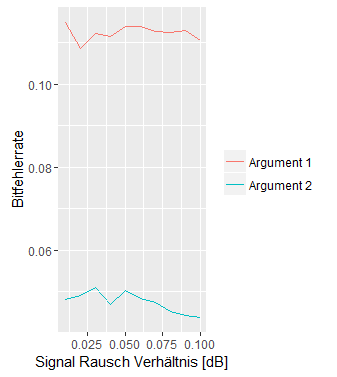
\includegraphics[width=\ScaleIfNeeded]{pictures/PlotSimulations}
\caption{Vergleich zweier Simulationen}
\label{pic:plotSimulations}
\end{figure}

Im Listing \ref{lst:plotSimulations} werden zwei verschiedene Simulationen mit unterschiedlichen Kodierern miteinander verglichen. Die erste Simulation stammt noch von Kapitel \ref{sec:example_simulations_turbo}, diese wird mit der Simulation des Standard-Kodierers verglichen. Die erstellte Grafik ist in Abbildung \ref{pic:plotSimulations} zu sehen, da ist deutlich zu erkennen, dass die erste Simulation klar die besseren Ergebnisse liefert.

\chapter{Fazit und Ausblick}
\label{chapter:conclusion}
\input{chapters/conclusion}

\cleardoublepage
\phantomsection
\addcontentsline{toc}{chapter}{\listfigurename}
\listoffigures
\cleardoublepage

\phantomsection
\addcontentsline{toc}{chapter}{Tabellenverzeichnis}
\printlist[tables]{lot}{}{\renewcommand\addvspace[1]{}\chapter*{Tabellenverzeichnis}}
\cleardoublepage

\phantomsection
\addcontentsline{toc}{chapter}{Funktionsverzeichnis}
\printlist[Funktionen]{lot}{}{\renewcommand\addvspace[1]{}\chapter*{Funktionsverzeichnis}}
\cleardoublepage

\phantomsection
\addcontentsline{toc}{chapter}{Listingverzeichnis}
\lstlistoflistings
\cleardoublepage
\phantomsection

\defbibheading{myheading}[Literatur]{%
  \chapter*{#1}}
\addcontentsline{toc}{chapter}{Literatur}
\pagestyle{plain}
\printbibliography[heading=myheading]

\end{document}
